\documentclass[12pt]{article}
\usepackage{amsfonts,amsthm,amsmath,amssymb}
\usepackage{hyperref}
\usepackage{fullpage}
\usepackage{graphicx}
\usepackage{indentfirst}
\usepackage[left=0.75in, right=0.75in]{geometry}
\linespread{1}	%1.5/1.2=1.25 for 1.5-space
\usepackage{titlesec}
\setlength{\parskip}{1em}
\usepackage{float}
\usepackage{caption}
\usepackage{subcaption}
\usepackage{listings}
\captionsetup{labelfont=bf}
\usepackage{pythonhighlight}


%\usepackage{biblatex}
%\bibliography{Bibliography}
%\iffalse
%\usepackage{biblatex}
%\addbibresource{Bibliography.bib}
%\addbibresource{Bibliography}
%\fi

\title{Applying Principal Component Analysis for Noise Reduction in Image Classification
}
\author{Andrew Duenner \\\texttt{duenner@mit.edu} \and Alex Kimn \\\texttt{akimn@mit.edu}}
\date{\today}

\begin{document}

\newcommand{\abs}[1]{\lvert#1\rvert}


\maketitle


%%%%%%%%%%%%%%%%%%%%%%%%%%%%%%%%%%%%%%%%%%%%%%%%%%%%%%%%%%%%%%%%%%%
%%%%%%%%%%%%%%%%%%%%%%%%%%%%%%%%%%%%%%%%%%%%%%%%%%%%%%%%%%%%%%%%%%%
\pagebreak
\tableofcontents

%%%%%%%%%%%%%%%%%%%%%%%%%%%%%%%%%%%%%%%%%%%%%%%%%%%%%%%%%%%%%%%%%%%
%%%%%%%%%%%%%%%%%%%%%%%%%%%%%%%%%%%%%%%%%%%%%%%%%%%%%%%%%%%%%%%%%%%
\pagebreak
\section{Introduction}\label{1}
As computer vision becomes more ubiquitous, expectations for speed and robustness continue to grow. This report focuses on the application of Principal component analysis (PCA) as a pre-processor to improve the robustness of image classifiers with respect to noisy data. Specifically, we consider convolutional neural networks (CNNs) trained on the MNIST dataset of handwritten characters. Methods for calculating principal components using singular value decomposition (SVD), eigenvector decomposition, and partial least squares minimization are introduced. 

Each method is implemented in Python and compared on the basis of \textit{Normalized Run-time}, \textit{Loss},  \textit{Error Rate}, and \textit{Mean Squared Error} (\textit{MSE}). Methods for calculating principal components are also compared on the basis of asymptotic operation count with respect to data set size, image size, and number of principal components used. Finally, the advantages and disadvantages of each method applied to image noise reduction are discussed and conclusions are presented.

%%%%%%%%%%%%%%%%%%%%%%%%%%%%%%%%%%%%%%%%%%%%%%%%%%%%%%%%%%%%%%%%%%%
%%%%%%%%%%%%%%%%%%%%%%%%%%%%%%%%%%%%%%%%%%%%%%%%%%%%%%%%%%%%%%%%%%%

\section{Overview of Principal Components}\label{2}
Principal component analysis is a mathematical transformation $X=TP^T$ that transforms a data set $X \in \mathbb{R}^{nxp}$ consisting of $n$ samples and $p$ variables with unknown correlation to a set of uncorrelated orthogonal loading vectors $P$  that map X to a matrix T of principal component scores. The transformation operates such that the first vector of P corresponds to the direction of the original data set with the largest variance \cite{jolliffe1986principal}. This property of principal components is useful for noise reduction in a data set as it allows for the correlated data to be separated from the uncorrelated data. X can be approximated as $\hat{X}$ by using the first k principle components such that $\hat{X}=T_kP_k^T$ with $X=\hat{X}+E$ and E an error term representing the remainder of X in the directions with the lowest correlation.

In \textbf{\hyperref[PCA]{Figure \ref*{PCA}}} on the following page, we present an example of PCA applied to the MNIST dataset. Each of the individual images is the result of projecting one noised digit onto the first $n$ principal components, which are extracted across the entirety of the noised dataset. 

\begin{figure}[H]
\begin{center}
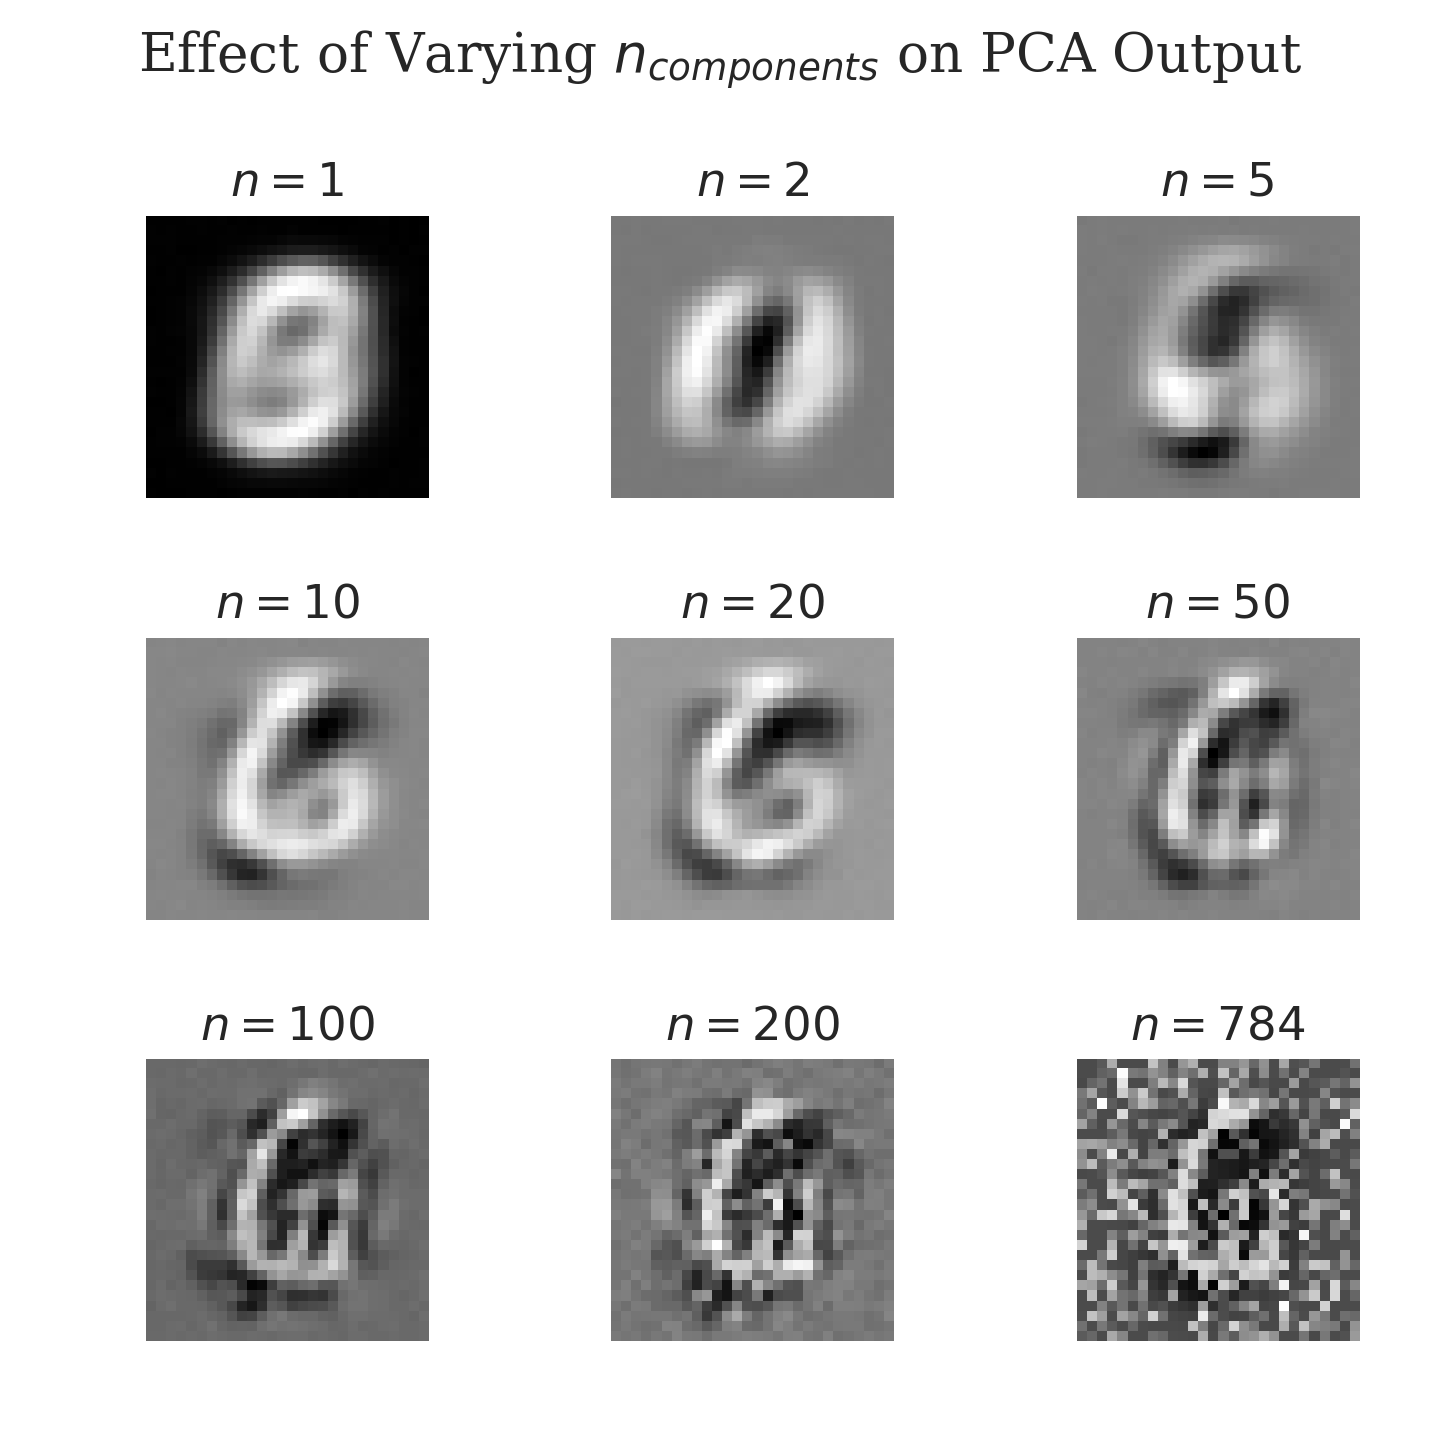
\includegraphics[width=\textwidth]{set_10.png}
\caption{Result of projecting a noised image representing a $6$ onto various numbers $n$ of principal components}
\label{PCA}
\end{center}
\end{figure}

%%%%%%%%%%%%%%%%%%%%%%%%%%%%%%%%%%%%%%%%%%%%%%%%%%%%%%%%%%%%%%%%%%%
%%%%%%%%%%%%%%%%%%%%%%%%%%%%%%%%%%%%%%%%%%%%%%%%%%%%%%%%%%%%%%%%%%%
\pagebreak
\section{Algorithms}\label{3}

%-----------------------------------------------------------------%
\subsection{NIPALS}\label{3.1}
The nonlinear iterative partial least squares (NIPALS) algorithm is an iterative algorithm that has the advantage of calculating principal components consecutively and with arbitrary accuracy. These attributes are desirable when the number of required principal components is uncertain or variable and the requirements on accuracy are somewhat relaxed. As such, it is an algorithm well-suited for pre-processing noised images quickly.

The NIPALS algorithm consists of an outer loop that calculates the $i^{th}$ next consecutive principal component . The outer loop begins with a guess of the $i^{th}$ score  vector. The initial value for $t_i$ may be set to the the $i^{th}$ column of the data set $X_i$ where i is the column index of the principal component being calculated \cite{risvik2007principal}. Next the inner product of $t_i$ is taken with respect to itself as $\lambda_i$ which represents the square of the magnitude of $t_i$. An inner loop next iteratively calculates the $i^{th}$ loading vector $p_i$, score vector $t_i$ and eigenvector $\lambda_i$. Within the inner loop $p_i$ is calculated by projecting the transpose of the data set $(X^T)$ onto the scores $t_i$. Vector $p_i$ is then normalized to prevent overflow. The scores vector $t_i$ is updated to be the projection of X onto p. A new $\lambda_{new}$ is calculated as the inner product of t with itself. If $|\lambda-\lambda_{new}|<tol$ the iterative inner loop breaks whereas otherwise $\lambda$ is set to $\lambda_{new}$.  After a number of iterations $t_i$ converges to the component score vector, $p_i$ converges to the component loading vector, and $\lambda_i$ converges to the $i^{th}$ largest eigenvalue of X. After the inner loop converges, the outer product of $t_i$ and $p_i$ is subtracted from X and the outer loop is repeated. The code snippet in Listing \ref{lst:NIPALS} below demonstrates an implementation of the NIPALS algorithm in Python with the Numba \cite{numba} package.

The computational complexity of the NIPALS algorithm is dominated by the matrix vector product operations used to project $X^T$ onto $t$ and $X$ onto P with $\mathcal{O}(\textbf{mn})$ complexity for a data set with $\textbf{m}$ samples and $\textbf{n}$ variables. Both of these operations take place within the inner loop of $k$ iterations to convergence and an outer loop of $\textbf{c}$ principal components. The entire algorithm is then $\mathcal{O}(k\textbf{c}\times\textbf{mn})$ where $\textbf{m}$ is images, $\textbf{n}$ is pixels per image, $\textbf{c}$ is number of principal components and $k$ is number of inner loop iterations necessary to reach desired accuracy.  
\pagebreak
\begin{lstlisting}[frame=none,caption={NIPALS Algorithm},captionpos=b,label=lst:NIPALS]
\end{lstlisting}
\begin{python}
# Nonlinear Iterative Partial Least Squares 
@jit(nopython=True) # Numba
def NIPALS(X, scores, loadings, lambdas, n_components, 
            threshold=1e-6, max_iter=200):

    # Iterate over each calculated component
    for i in range(n_components):

        t = X[:, i]
        lambda_ = np.dot(t, t) 

        # Iterate until convergence
        for j in range(max_iter):

            # Compute loadings
            p = np.dot(X.T, t)
            p /= lambda_
            loadings[:, i] = p

            p /= np.linalg.norm(p)
    
            # Project X onto p to find score vector t
            t = np.dot(X, p)
            t /= np.dot(p, p)
            scores[:, i] = t
      
            lambda_n = np.dot(t, t)

            # Add score vector to matrix of score vectors
            lambdas[i] = lambda_n

            # Check for convergence
            diff = np.abs(lambda_ - lambda_n)

            if diff < threshold:
                break

            lambda_ = lambda_n
           
        # Update X
        X -= np.outer(t, p) 
\end{python}


%-----------------------------------------------------------------%
\subsection{SVD}\label{3.2}
Singular Value Decomposition is a commonly implemented method for calculating principal components \cite{oliphant2009numpy} \cite{scikit-learn}. The SVD transformation satisfies the equality $X=U \Sigma V^*$ for $X \in \mathbb{C}^{m,n}$, where
$ U\in \mathbb{C}^{m,n}$ is a unitary matrix representing the left singular vectors of X, $ V\in \mathbb{C}^{n,n}$ is a unitary matrix representing the right singular vectors of X, and $\Sigma \in \mathbb{C}^{m,n}$ is a diagonal matrix of the singular values of X \cite{trefethen1997numerical}. The principal component score vectors $t_i$ of a mean-centered dataset $X$ can be calculated as $U \Sigma $ and the loading vectors are $VX$ \cite{madsen2004singular}. 

SVD decomposition was chosen as a benchmark algorithm to highlight the computational complexity implications of calculating only a few principal components versus calculating all components at once via a method such as SVD. A common algorithm for calculating singular value decomposition of a matrix is the gebrd algorithm in LAPACK. The gebrd algorithm calculates all of the singular values and singular vectors simultaneously with $\mathcal{O}\big( \frac{4}{3}\textbf{n}^2(3\textbf{m} - \textbf{n}) \big)$ complexity \cite{intelmath}. Thus the NIPALS algorithm is computationally less complex than calculating SVD when $\frac{4}{3}\textbf{n}(3\textbf{m} - \textbf{n})>(k\textbf{c}\times\textbf{m})$.  \\ An implementation of principal component analysis by SVD using Python and the Numba package \cite{numba} is given below in code listing \ref{lst:SVD}.

\begin{lstlisting}[frame=none,caption={Calculating Principal Components with SVD},captionpos=b,label=lst:SVD]
\end{lstlisting}

\begin{python}
@jit(nopython=True) # Numba
def SVD(X, scores, loadings, lambdas, n_components):

    u, s, vt = np.linalg.svd(X, full_matrices=False)
    m = X.shape[0]

    loadings[:] = (vt.T)[:, 0:n_components]
    scores[:] = np.dot(u, np.diag(s))[:,0:n_components]
    lambdas[:] = np.dot(s, s)
    lambdas /= (m - 1)
\end{python}


%-----------------------------------------------------------------%
\subsection{Eigenvector Decomposition (Simultaneous Iteration)}\label{3.3}
Eigenvector decomposition provides yet another method for calculating principal components. An iterative method for simultaneously calculating the the largest \textbf{c} eigenvalues $\lambda_c$ and eigenvectors $\Lambda_c$ was selected as a benchmark algorithm to provide a comparative basis for iteratively calculating principal components sequentially as in NIPALS versus calculating them simultaneously. 

Calculating principle components with eigenvector decomposition starts with calculation of the covariance $C \in \mathbf{R}^{n,n}$ of the zero-mean data set $X^T \in \mathbf{R}^{n,m}$ represented such that the rows \textbf{n} are variables (pixels) and the columns \textbf{m} are samples (images).  
$$C=\frac{1}{n-1}X^TX$$
Calculating the covariance matrix is of $\mathcal{O}(\textbf{mn}^2)$. Note that for datasets with large images it may be unfeasible to calculate the pixel covariance and store it in memory. MNIST images with 28x28 pixels represented as int16 values on one color channel can be represented in an uncomprssed form as a 9.8MB file whereas a VGA image with 640x480 pixels requires 188GB of in-memory storage.      

Eigenvector decomposition is a transformation of the form $C=Q \lambda Q'$ where Q are the eigenvectors of C and $\lambda$ are the eigenvalues. Simultaneous iteration solves for the $k$ largest eigenvalue eigenvector pairs simultaneously by repeatedly multiplying the covariance matrix $C \in \mathbb{R}^{n,n}$ by a matrix $Q^{n,c}$ which is initialized with random values. Matrix $Q$ converges to the $c$ largest eigenvectors of the covariance matrix $C$ \cite{trefethen1997numerical}. In order to prevent the largest eigenvector from dominating all columns in $Q$, Matrix A is reorthogonalized every iteration using the modified gram-schmidt procedure adapted from \cite{srinivasan}. $Q_0$ is then set to Q and the value of Q is tested for convergence. Convergence conditions are considered satisfied when the orthogonal projection of $Q$ onto $Q_0$ is sufficiently small as discussed in \cite{arbenz2012lecture}. 
$$ \|(I-Q_kQ_k^T)Q_{k-1}\|<tol$$

The principal component score matrix T and loading vector P can be constructed from the covariance C,  Eigenvectors $Q$ and Eigenvalues $R$ as follows.
$$T=QC$$
$$P=V$$

The outer loop of the simultaneous power iteration algorithm is dominated in computational complexity by the multiplication of C with Q which is $\mathcal{O}(\textbf{cn}^2)$ and the inner loop in which modified gram schmidt is used to orthogonalize A is of $\mathcal{O}(\textbf{2nc}^2)$. The total complexity is then approximately $\mathcal{O}((2\textbf{nc}^2+\textbf{n}^2\textbf{c})k$ and is quadratic with the number of pixels chosen for simultaneous computation. $\lim_{c \to n} \mathcal{O}((2\textbf{nc}^2+\textbf{n}^2\textbf{c})k=3n^3k$ the complexity is cubic with n and as such this method should be used for low c. Code listing \ref{lst:simuliter} below shows a numpy implementation of simultaneous iteration with orthogonalization at each step by MGS. 
\pagebreak
\begin{lstlisting}[frame=none,caption={Calculating Principal Components with Eigenvalue Decomposition via Simultaneous Power Iteration},captionpos=b,label=lst:simuliter]
\end{lstlisting}
\begin{python}
@jit(nopython=True) # Numba
def SI(X, Q, Q_o, R, I, threshold=1e-6, max_iter=200): 

    for k in range(max_iter):

        A = operator.matmul(C, Q)

        Q_o[:] = Q

        _MGS(A, Q, R)

        delta = operator.matmul(I - np.dot(Q, Q.T), Q_o)
       
        if np.linalg.norm(delta) <= threshold:
            break
            
@jit(nopython=True) # Numba
def MGS(A, Q, R):

    (m, n) = A.shape

    for k in range(n):

        R[k, k] = np.sqrt(np.dot(A[:, k], A[:, k]))
        Q[:, k] = A[:, k] / R[k, k]

        for j in range (k + 1, n):

            R[k, j] = np.dot(Q[:, k].T, A[:, j])
            A[:, j] -= R[k, j] * Q[:, k]
\end{python}

%-----------------------------------------------------------------%
\subsection{GPU Paralellization}\label{3.4}

Consumer grade graphics processing units have been released with the capability to perform parallel computation of floating point arithmetic at high speed. In this study GPU hardware was used for the neural network classifier and so it was a natural extension to implement the image preconditioner in GPU-executable code as well. It was hypothesized that at least some reduction in computation time could be achieved by taking advantage of parallelization of matrix operations. 

PyTorch was used as a high-end language to execute the NIPALS algorithm on a consumer-grade gaming GPU. Conversion from numpy to PyTorch proved to be a trivial development exercise and the resulting algorithm ran significantly faster on the GPU when compared to execution on a CPU. Figure \ref{parallelization} shows a comparison of the CPU and GPU implemented time to process a range of dataset sample sizes \textbf{n} . The number of components calculated, $n_{components}$, is set to $5$ and full images were used ($n_{pixels}=784$). 

\begin{figure}[H]
\begin{center}
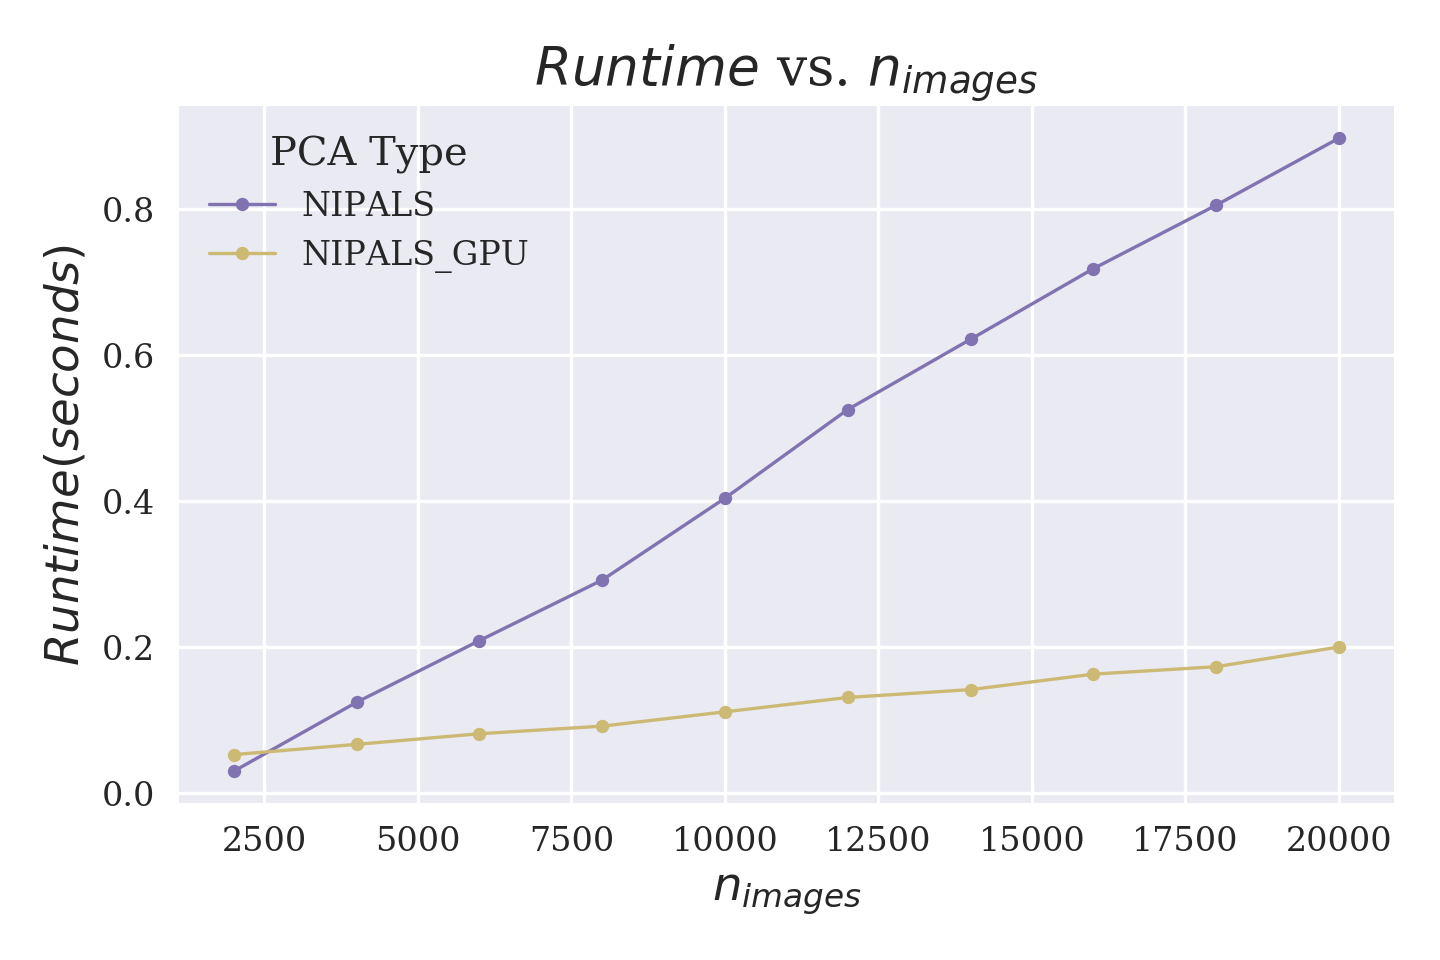
\includegraphics[width=\textwidth]{U_GPU.png}
\caption{Runtimes of the CPU- and GPU-implemented versions of the NIPALS algorithms as observed on a GTX 1080}
\label{parallelization}
\end{center}
\end{figure}

The data shows that runtime on the GPU is a factor of 4-5 times less than that of the CPU. Note that the GPU advantage is dependent on the number of images and for smaller datasets the CPU implementation is faster. This is likely due to the overhead associated with memory bandwidth and transfer between RAM on the CPU and GPU.

%%%%%%%%%%%%%%%%%%%%%%%%%%%%%%%%%%%%%%%%%%%%%%%%%%%%%%%%%%%%%%%%%%%
%%%%%%%%%%%%%%%%%%%%%%%%%%%%%%%%%%%%%%%%%%%%%%%%%%%%%%%%%%%%%%%%%%%
\pagebreak
\section{Methodology} \label{4}

    In order to assess the relative performance of each of the algorithms, we measure four separate metrics: \textit{Normalized Run-time}, \textit{Loss},  \textit{Error Rate}, and \textit{Mean Squared Error} (\textit{MSE}). \textbf{\hyperref[methodology]{Figure \ref*{methodology}}} below provides an overview of how this is achieved.
    
    \begin{figure}[H]
    \begin{center}
    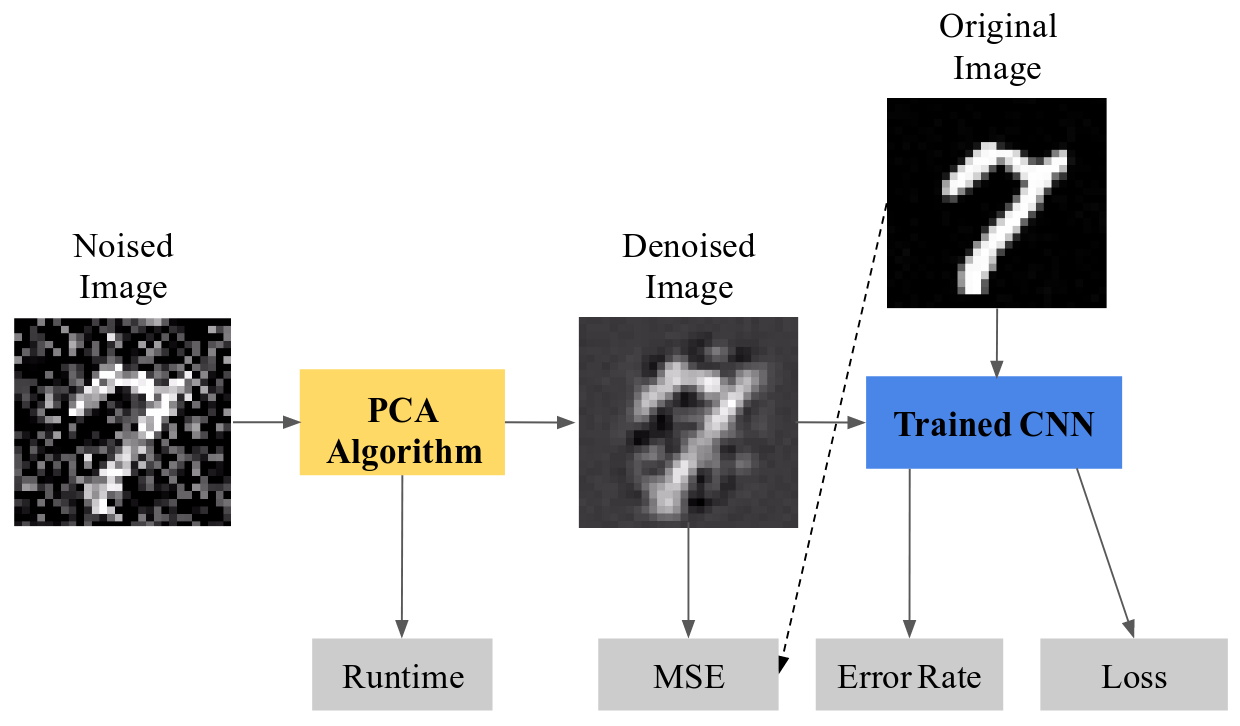
\includegraphics[width=\textwidth]{Methodology.png}
    \caption{A flow chart of the bench-marking process}
    \label{methodology}
    \end{center}
    \end{figure}
    
    A fair assessment of the relative cost of running each algorithm is rather difficult to obtain. While we implement all three using only the Python library \textit{NumPy},its built-in functions use a variety of different back-ends. Therefore, we wrap each of the \textit{NumPy} implementations inside \textit{Numba} to unify the back-ends used, making it so that all three algorithms are compiled by LLVM and run as machine code. 
    
    Moreover, since neither \textit{NumPy} nor \textit{Numba} offer methods to directly determine the number of used floating point operations, we resort to using \textit{Normalized Run-time} instead as a proxy for cost. Of course, we cannot guarantee that raw runtimes across methods are proportional to relative cost. However, given the unified \textit{Numba} back-end, we should expect that the runtimes of different instances of the same method are proportional to computational complexity. Hence, if these runtimes are then normalized at some fixed value of the independent variable, we can compare their relative trajectory across that variable. Using this, we evaluate the computational complexities of the three algorithms on two values of dataset size, the number of images, $n_{images}$, and the number of pixels per image, $n_{pixels}$, as well as the number of components extracted, $n_{components}$.
    
    In addition to the algorithms' computational costs, we also measure the quality of their output. In the context of the original problem, higher quality outputs should result in an improvement in the classifier's discriminatory ability. Since this quality depends on $n_{components}$, we test each PCA algorithm on a set of $20$ $n_{components}$ values ranging from $10$ to $680$. Additionally, we apply each of these $20$ variants to $8$ different noised datasets (with mean noise mask magnitude ranging from $\mu_{noise} = 10$ to $80$), resulting in a total of $160$ different de-noised outputs for each algorithm. From there, we run these outputs through a set of five CNN classifiers, each trained using $PyTorch$ on the same un-noised training data, and record the average \textit{Loss} and average \textit{Error Rate} that is observed. 
    
    Finally, noting that the trained classifiers are all unique and thus introduce additional variance into the problem, we select an objective evaluation of image quality. In particular, for each noised image $N_i$ in a noised dataset (where $i$ is its index in the set), we set the image it was derived from, $O_i$ as the ground truth and determine the mean squared error of the de-noised image, $D_i$ with respect to it. These values are then averaged across the entire set to obtain the final value of \textit{MSE}, as shown below:
    
    $$ \textit{MSE} = \frac{1}{n_{images}}\frac{1}{n_{pixels}}\sum_{i=1}^{n_{images}}\sum_{j=1}^{n_{pixels}}(D_i[j] - O_i[j])^2$$
    
    As with \textit{Loss} and \textit{Error Rate} we calculate \textit{MSE} for each of the $8$ magnitude of noise and and several different values for $n_{components}$.
   
%%%%%%%%%%%%%%%%%%%%%%%%%%%%%%%%%%%%%%%%%%%%%%%%%%%%%%%%%%%%%%%%%%%
%%%%%%%%%%%%%%%%%%%%%%%%%%%%%%%%%%%%%%%%%%%%%%%%%%%%%%%%%%%%%%%%%%%

\section{Algorithm Benchmark Results}\label{5}

%-----------------------------------------------------------------%
\subsection{Normalized Runtime}\label{5.1}

Before analyzing the results obtained from testing the PCA algorithms, we analyze the general asymptotic time complexity of each of the algorithms as they are implemented in \textit{Numba}. Please refer back to sections \textbf{\hyperref[3.1]{3.1}}, \textbf{\hyperref[3.2]{3.2}}, and \textbf{\hyperref[3.3]{3.3}} for the raw code used for each algorithm.

\subsubsection{Asymptotic Complexity}\label{5.1.1}

We note that the computational complexity of the three PCA algorithms is primarily determined by three values: $\textbf{m} == n_{images}$, $\textbf{n} == n_{pixels}$, and $\textbf{c} == n_{components}$.  Given these variables, we can estimate the asymptotic complexity of each as follows:

\textbf{\hyperref[3.1]{NIPALS}}: The operation count of the inner loop is dominated by the calculation of the two dot products involving the data array $X$. Knowing that $X$ has size $(\textbf{m}, \textbf{n})$, we can deduce that both of these function calls are $\mathcal{O}(\textbf{m}\textbf{n})$. Then, taking into consideration the two loops, we find that the NIPALS method is $\mathcal{O}(k \times \textbf{c} \times \textbf{m}\textbf{n})$, where $k<=max\_iter$ represents the number of inner loop iterations needed for convergence.

\textbf{\hyperref[3.2]{SVD}}: The method's cost is dominated by producing the SVD of the original data, which is size $(\textbf{m}, \textbf{n})$. Hence, we expect this method to have time complexity $\mathcal{O}(\textbf{n}^2 \textbf{m} ])$. Note that since the algorithm computes all the principal components by default, the runtime has no dependence on $\textbf{c}$

\textbf{\hyperref[3.3]{Simultaneous Iteration}}: The majority of the computation for each iteration is done to complete a Modified Gram-Schmidt (MGS) orthogonalization. Given that the inputted matrix $X$ has dimensions $(\textbf{n}, \textbf{n})$, we determine that the complexity of each inner loop within the MGS iterations is $\mathcal{O}(\textbf{n})$. Since both the inner and outer loops of MGS are called $\textbf{c}$ times, each MGS call has time complexity $\mathcal{O}(\textbf{n}\textbf{c}^2)$. Note that since the size of the input to the algorithm has no relation to the number of images inputted, the runtime has no dependence on $\textbf{m}$. Finally, as with NIPALS above, Simultaneous Iteration also loops at $k <=max\_iter$ times until convergence. Hence we find that this algorithm is $\mathcal{O}(k \times \textbf{n}\textbf{c}^2)$

To confirm this analysis, we vary all three of \textbf{m}, \textbf{n}, and \textbf{c} and measure the resulting \textit{Normalized Runtime} of each of the algorithms as they are applied to a set of $70000$ images noised with a mask of magnitude $30$.

\subsubsection{Runtime and $\textbf{m} == n_{images}$}\label{5.1.2}

The first variable we examine is $\textbf{m} == n_{images}$. In this first test, full images are used ($n_{pixels}=784$), and $n_{components}$ is set as $50$. $n_{images}$ is varied from $100$ to $1000$ and $15$ trials are run for each of the algorithms. The median value of the resulting runtimes is then taken as the representative value. Also, the images used in each trial are randomly selected from the dataset to ensure that representative values of $k$ are obtained for both \textbf{\hyperref[3.1]{NIPALS}} and \textbf{\hyperref[3.3]{Simultaneous Iteration}}. 

The results of this test are shown in a raw and normalized form below in \textbf{\hyperref[UPixels]{Figures \ref*{UImages}}} and \textbf{\hyperref[NPixels]{\ref*{NImages}}}, respectively. Note that in the normalized graph, all three methods are chosen to have runtime $1$ at $n_{images} = 100$.

\begin{figure}[H]
\centering
\begin{minipage}{.45\textwidth}
  \centering
  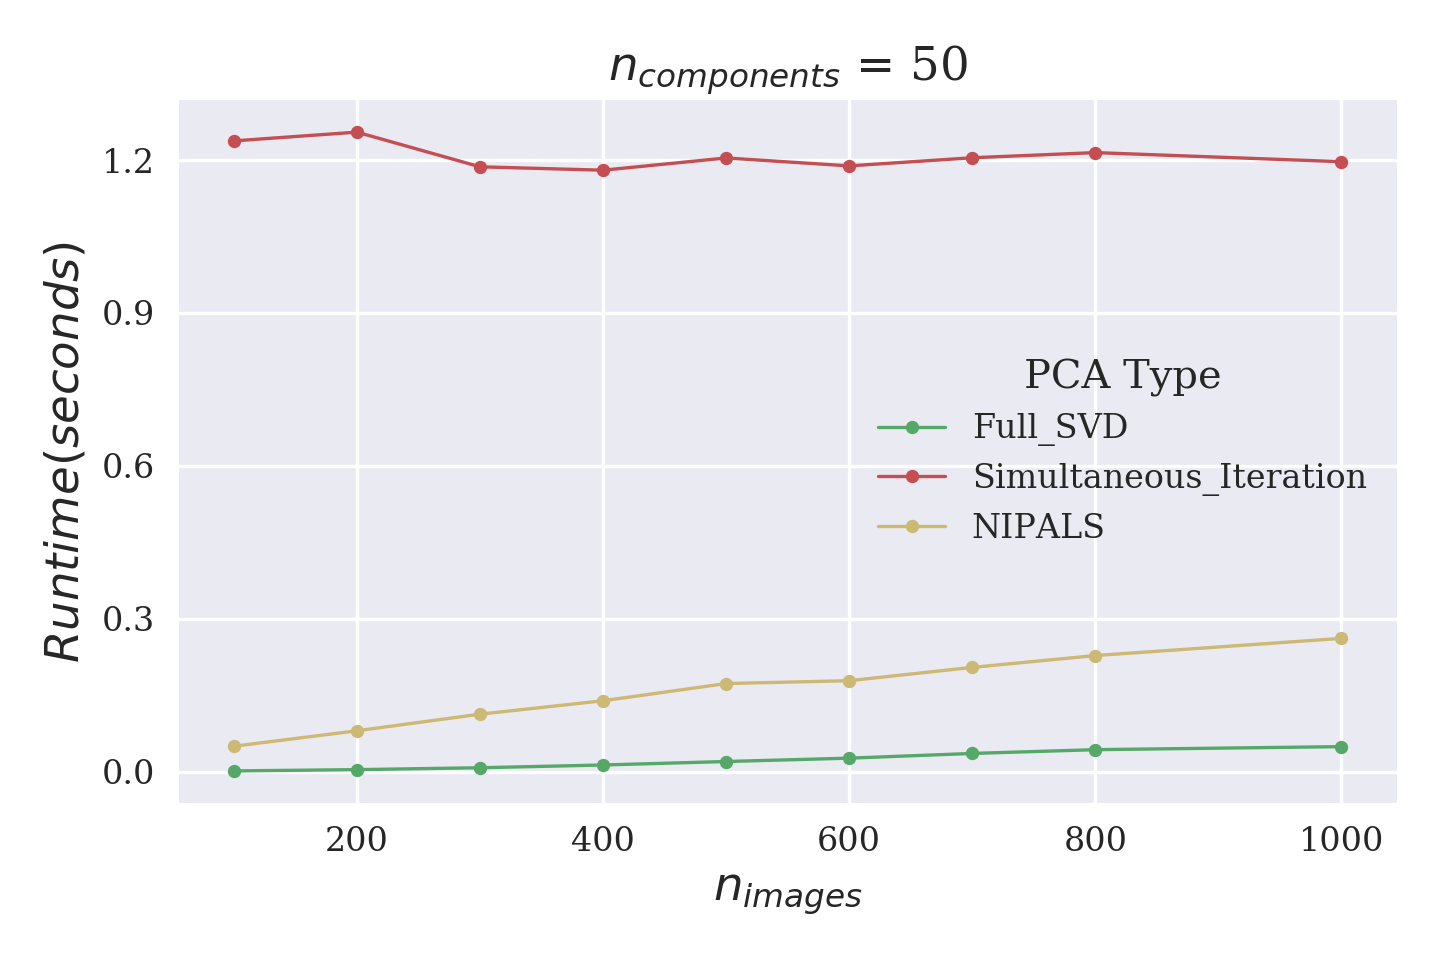
\includegraphics[width=\linewidth]{UImages.png}
  \captionof{figure}{Unnormalized runtime behavior of PCA algorithms when $n_{images}$ is varied.}
  \label{UImages}
\end{minipage}%
\quad
\begin{minipage}{.45\textwidth}
  \centering
  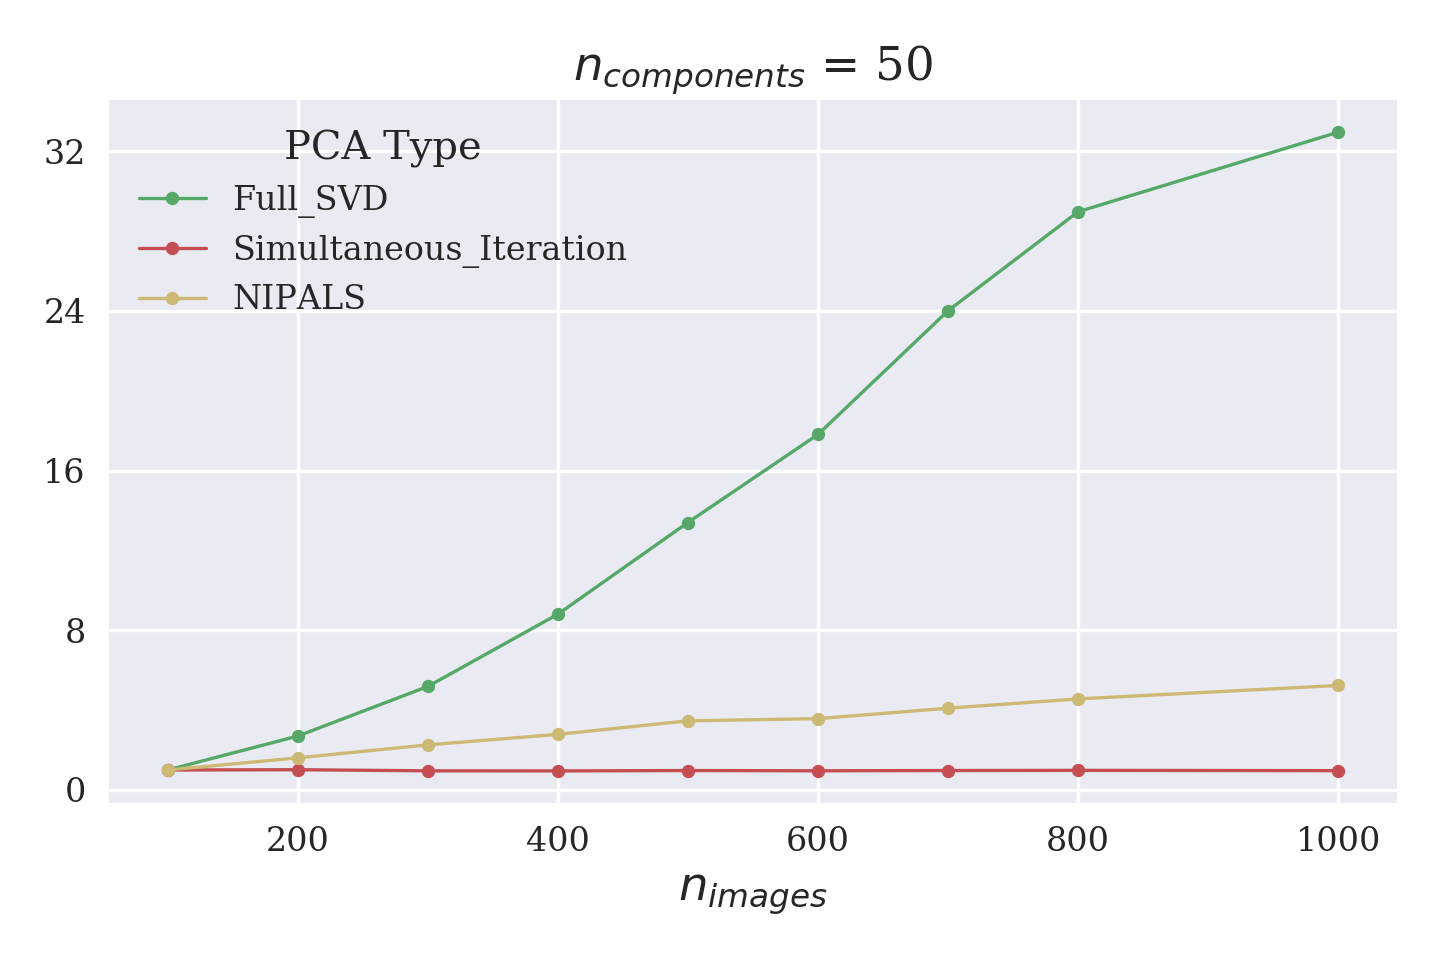
\includegraphics[width=\linewidth]{NImages.png}
  \captionof{figure}{Normalized runtime behavior of PCA algorithms when $n_{images}$ is varied.}
  \label{NImages}
\end{minipage}
\end{figure}

From our time complexity analysis, we expect to see a linearly increasing runtime for both \textbf{\hyperref[3.1]{NIPALS}} and \textbf{\hyperref[3.2]{SVD}}. And indeed, this trend is clearly visible on the normalized graph. Moreover, our expectation of constant runtime for the \textbf{\hyperref[3.3]{Simultaneous Iteration}} algorithm is also confirmed by the data. 

These results suggest that for datasets in which the number of unique samples far exceeds the number of components calculated, the \textbf{\hyperref[3.3]{Simultaneous Iteration}} variant of PCA may be the most cost-efficient. However, we note that for the MNIST problem we explore, the number of computed components is usually quite large, and the number of images is relatively small, making \textbf{\hyperref[3.2]{SVD}} the most efficient. 

\subsubsection{Runtime and $\textbf{n} == n_{pixels}$}\label{5.1.3}

Next, we show how varying the value of $\textbf{n} == n_{pixels}$ affects the time cost of the algorithms. In this test, we fix $n_{images}$ to be $5000$ and $n_{components}$ to be $5$, and vary $n_{pixels}$ from $20$ to $320$. We run $25$ trials for each of the algorithms, selecting the median value as the representative value. As before, we randomly select the images (and also pixels) used in each individual trial to ensure that we obtain representative values of $k$. 

The results of this test are shown in a raw and normalized form below in \textbf{\hyperref[UPixels]{Figures \ref*{UPixels}}} and \textbf{\hyperref[NPixels]{\ref*{NPixels}}}, respectively. Note that in the normalized graph, all three methods are chosen to have runtime $1$ at $n_{pixels} = 20$.

\begin{figure}[H]
\centering
\begin{minipage}{.45\textwidth}
  \centering
  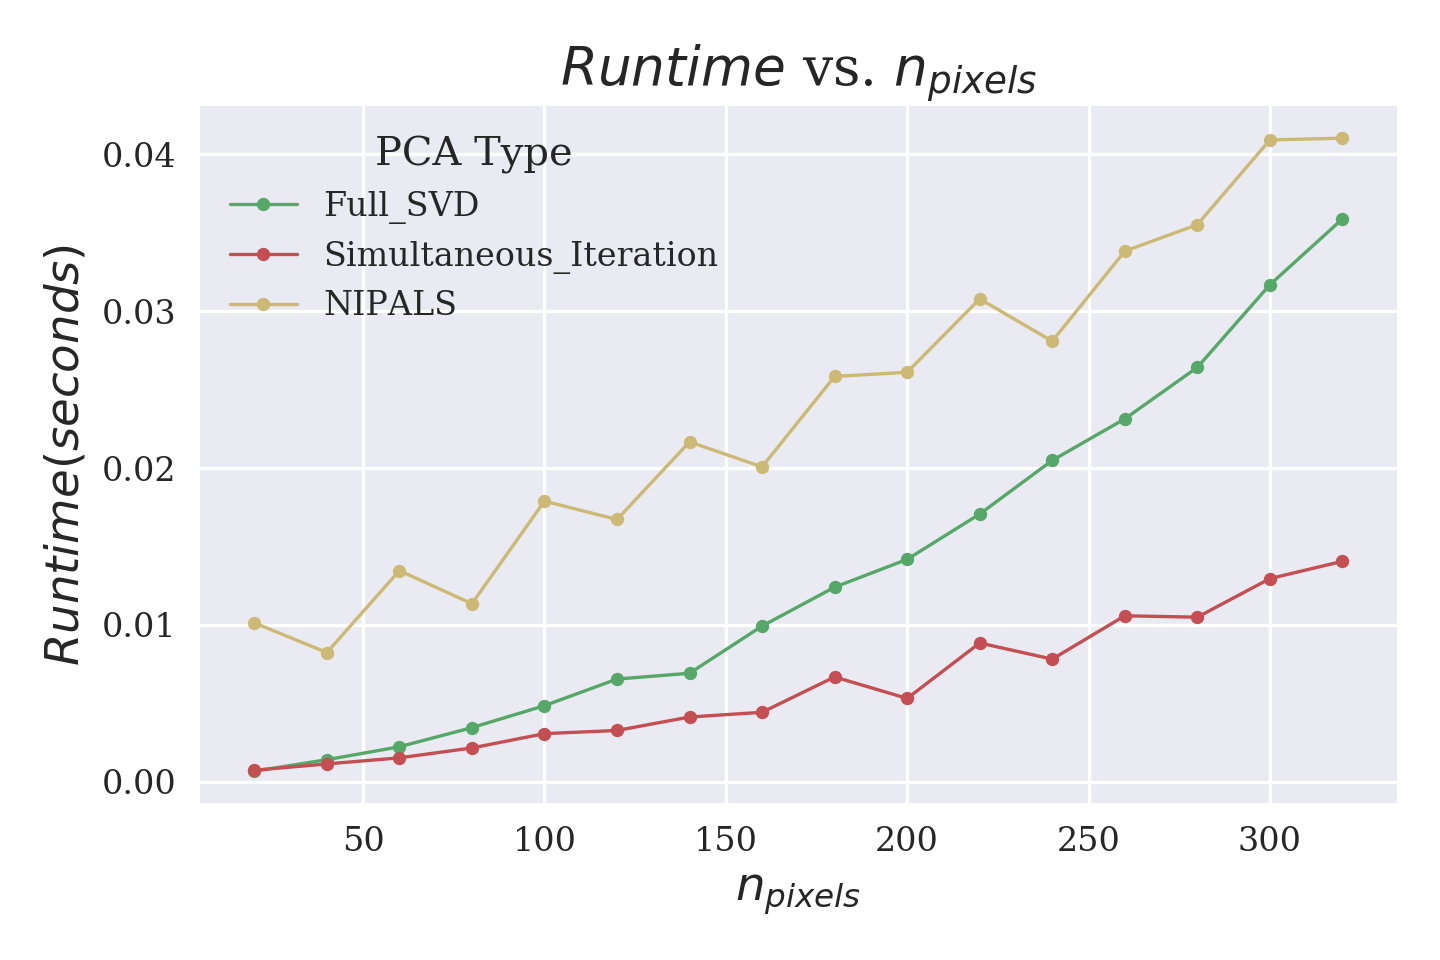
\includegraphics[width=\linewidth]{U_Pixels.png}
  \captionof{figure}{Unnormalized runtime behavior of PCA algorithms when $n_{pixels}$ is varied.}
  \label{UPixels}
\end{minipage}%
\quad
\begin{minipage}{.45\textwidth}
  \centering
  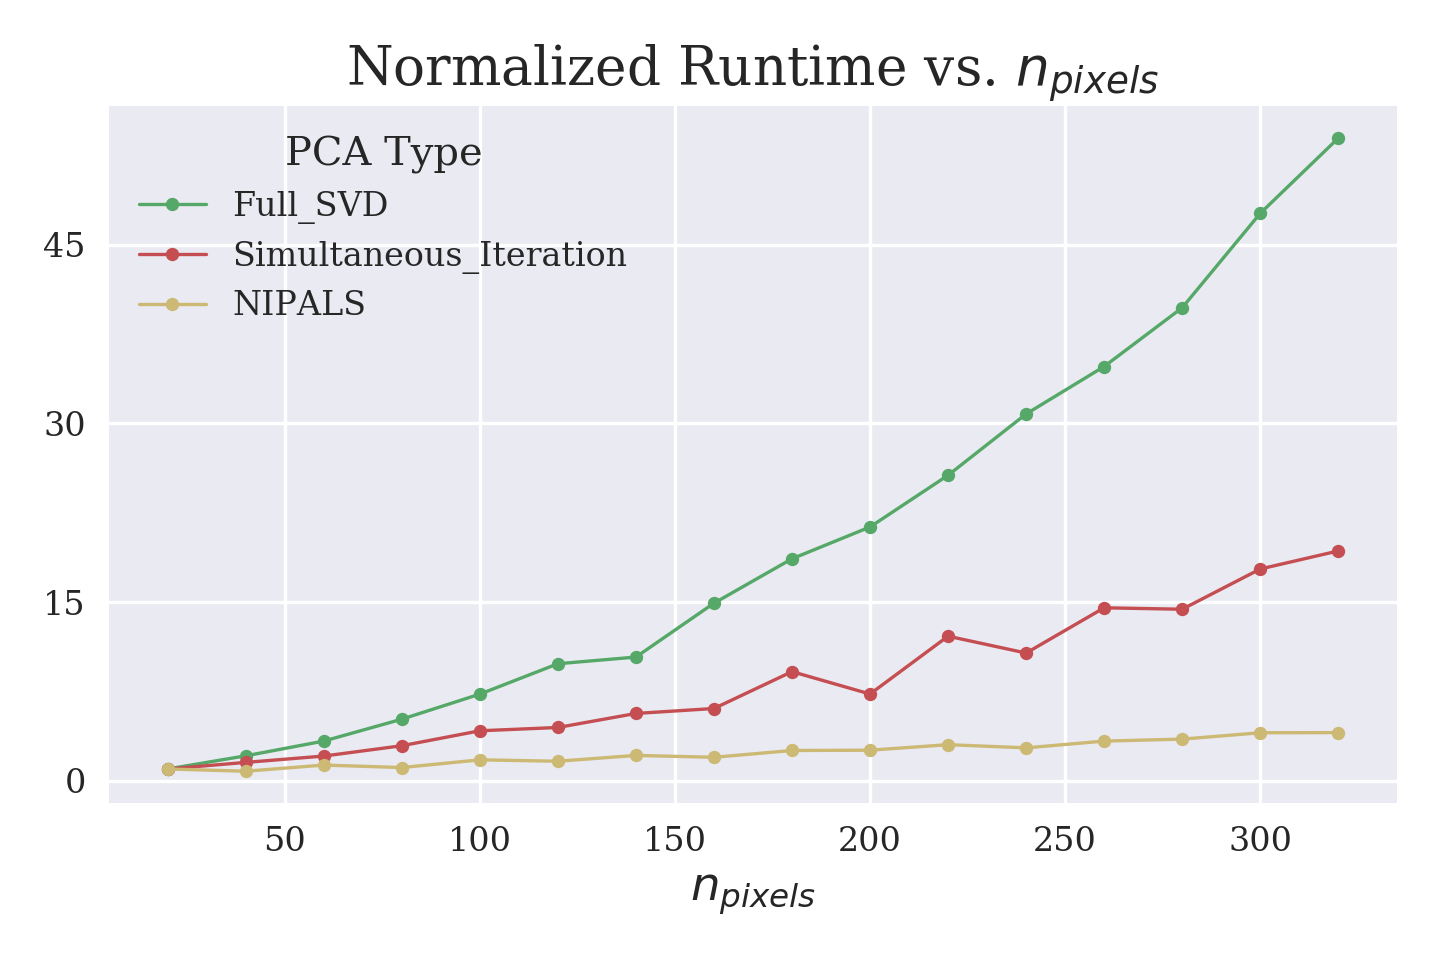
\includegraphics[width=\linewidth]{N_Pixels.png}
  \captionof{figure}{Normalized runtime behavior of PCA algorithms when $n_{pixels}$ is varied.}
  \label{NPixels}
\end{minipage}
\end{figure}

Using the complexity analysis above, we predict \textbf{\hyperref[3.2]{SVD}} to have quadratic complexity in $n_{pixels}$, which the data appears to confirm. Moreover, our expectations of linear runtimes for both \textbf{\hyperref[3.1]{NIPALS}} and \textbf{\hyperref[3.3]{Simultaneous Iteration}} are also supported by the graphs. 

These data suggest that for datasets with large image sizes, unlike the MNIST dataset, $SVD$ will no longer be the most cost-efficient algorithm. In particular, for datasets with many big images, it is likely that \textbf{\hyperref[3.3]{Simultaneous Iteration}} will be the most cost-efficient. On the other hand, if the images are sufficiently large and the number of components needed to be computed is relatively high, \textbf{\hyperref[3.1]{NIPALS}} may become the most efficient.

\subsubsection{Runtime and $\textbf{c} == n_{components}$}\label{5.1.4}

Finally, we analyze $n_{components}$. Here, we fix $n_{images}$ to be $1000$ and again use full images (i.e. $n_{pixels}$=784). We run $15$ trials, randomly selecting the images and taking the median runtime as the representative. 

The results of this test are shown in a raw and normalized form below in \textbf{\hyperref[UPixels]{Figures \ref*{UComponents}}} and \textbf{\hyperref[NPixels]{\ref*{NComponents}}}, respectively. Note that in the normalized graph, all three methods are chosen to have runtime $1$ at $n_{components} = 10$.

\begin{figure}[H]
\centering
\begin{minipage}{.45\textwidth}
  \centering
  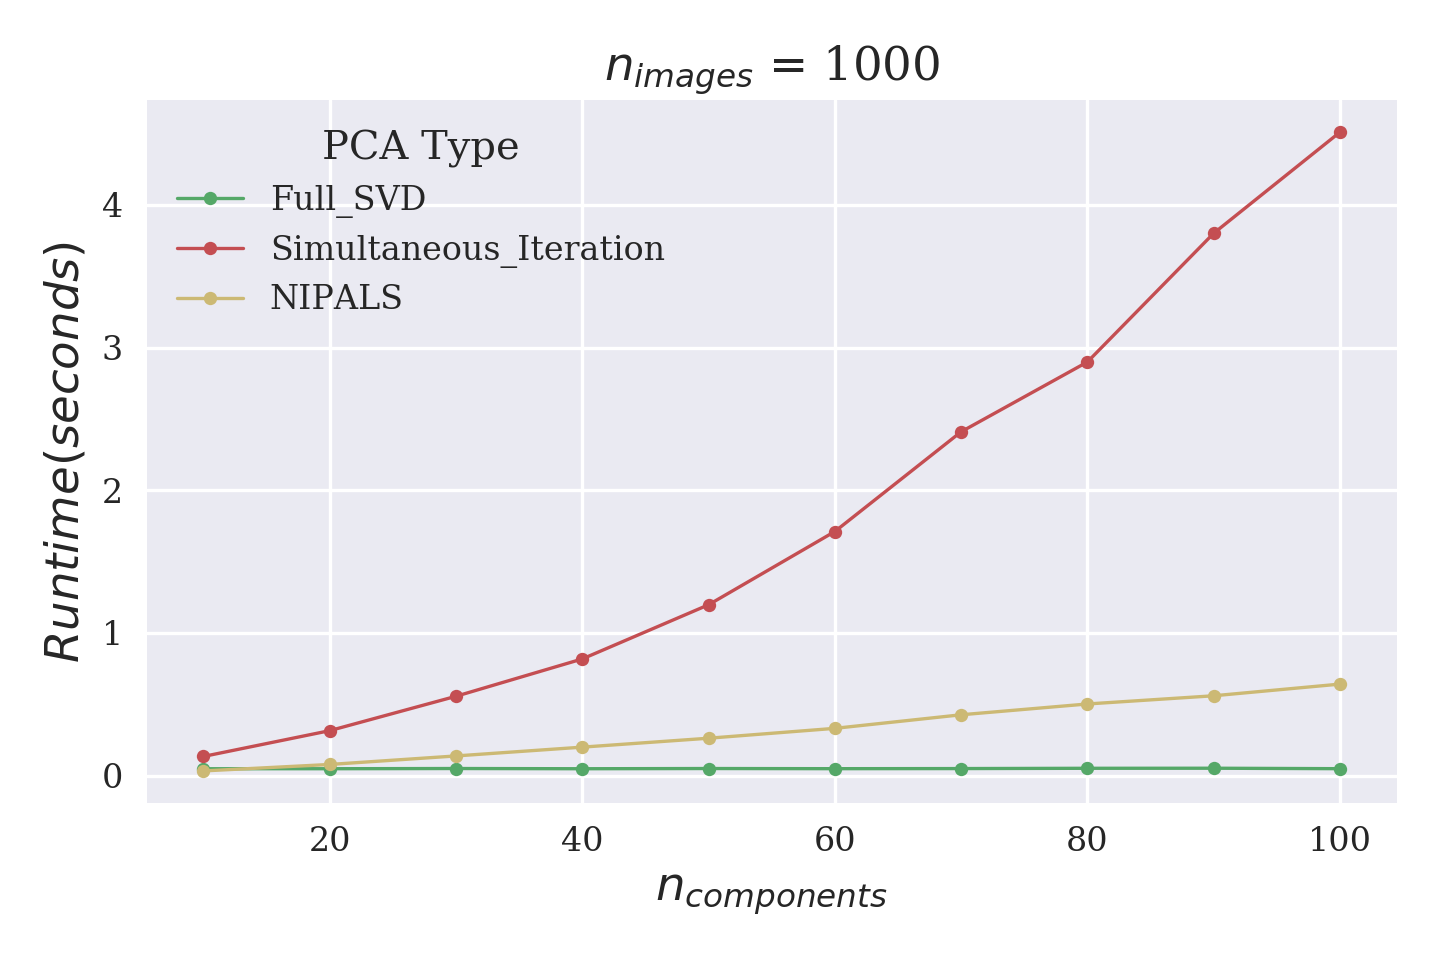
\includegraphics[width=\linewidth]{UComponents.png}
  \captionof{figure}{Unnormalized runtime behavior of PCA algorithms when $n_{images}$ is varied.}
  \label{UComponents}
\end{minipage}%
\quad
\begin{minipage}{.45\textwidth}
  \centering
  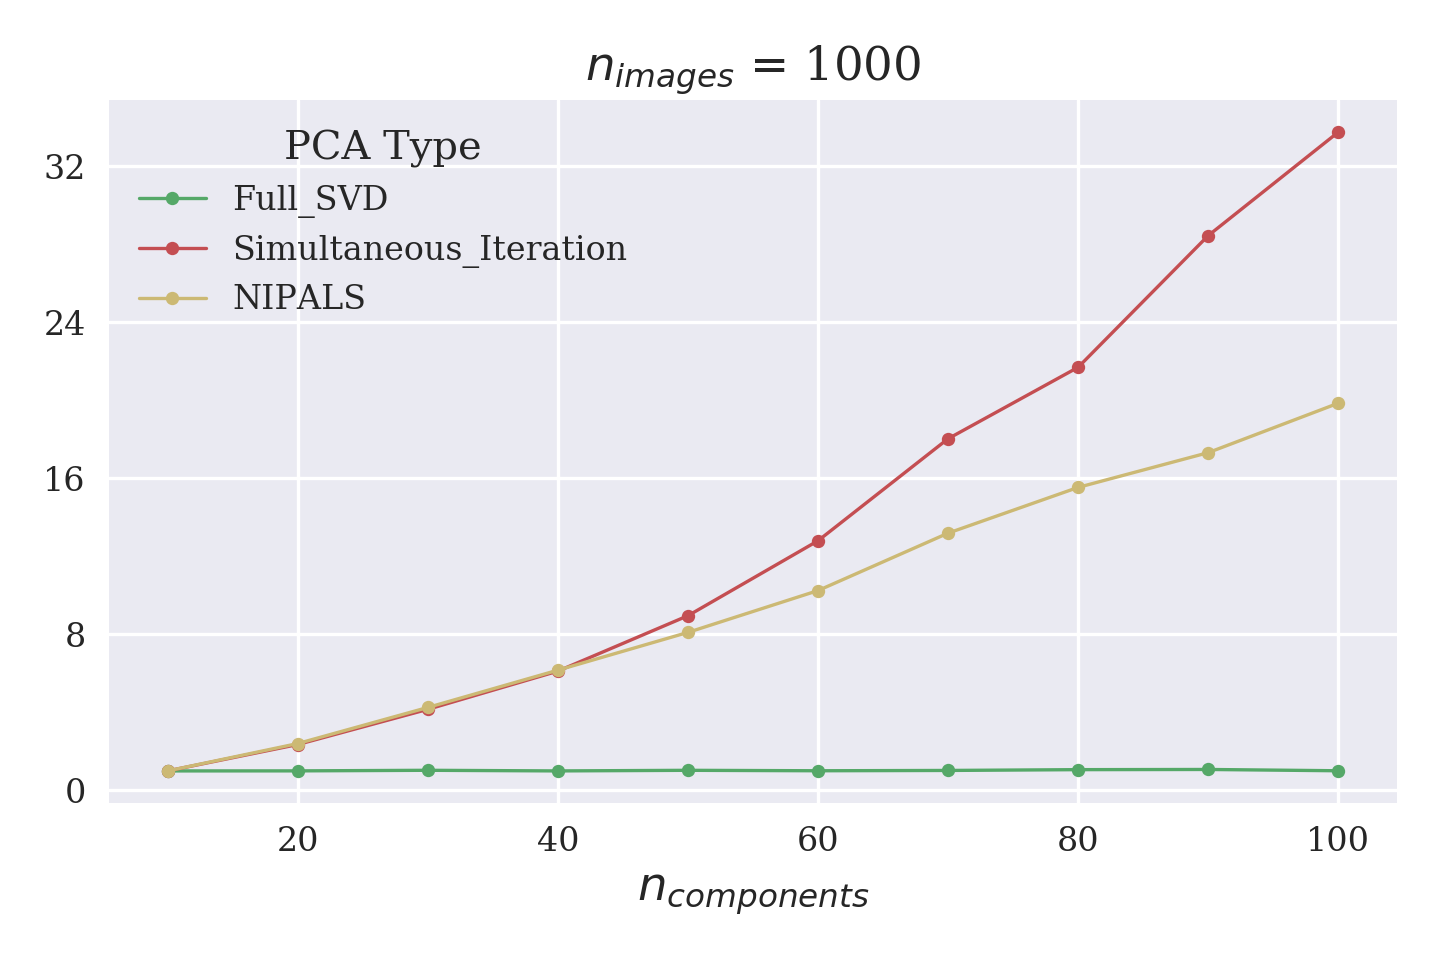
\includegraphics[width=\linewidth]{NComponents.png}
  \captionof{figure}{Normalized runtime behavior of PCA algorithms when $n_{images}$ is varied.}
  \label{NComponents}
\end{minipage}
\end{figure}

The data confirms the predicted linear relation between the cost and $n_{components}$ for \textbf{\hyperref[3.1]{NIPALS}}. The quadratic complexity of \textbf{\hyperref[3.3]{Simultaneous Iteration}} is also clearly visible in the normalized graph. Finally, the data confirms that the cost of \textbf{\hyperref[3.2]{SVD}} does not depend at all on the number components extracted.

These data reinforce the conclusions drawn in the previous two sections. In particular, it is again clear that for problems in which large numbers of principal components must be computed, \textbf{\hyperref[3.2]{SVD}} will likely be the most efficient. 

\subsubsection{Overview}\label{5.1.5}

In general, the above assessments confirm the theoretical complexities of three three PCA algorithms. However, this means that the relationship between computational and the data parameters differs for all three algorithms. And if we extrapolate the complexity relationships observed to additional datasets and problems, we should find that the computationally cheapest PCA algorithm may vary. 

In particular, we would expect \textbf{\hyperref[3.1]{NIPALS}} to excel in problems where $n_{components}$ is low and the total data size of the problem is sufficiently large. However, if the number of unique data samples is sufficiently large, we would expect \textbf{\hyperref[3.3]{Simultaneous Iteration}} to be the most efficient. Finally, for problems like image de-noising, where the the value of $n_{components}$ is high and the dataset size relatively small, we should expect to see that \textbf{\hyperref[3.2]{SVD}} be the most efficient.
Indeed, as observed in the following sections, de-noising the MNIST dataset often required up to $100$ principal components to achieve the best noise reduction, And as shown by the unnormalized graphs above, the raw runtime for \textbf{\hyperref[3.2]{SVD}} was often only a fraction of that of the other two methods. 

%-----------------------------------------------------------------%
\subsection{Mean Squared Error}\label{5.2}

The obtained values of \textit{MSE} for both the lowest noise ($\mu_{noise}=10$) and highest noise ($\mu_{noise}=80$) datasets are shown below in \textbf{\hyperref[Noise10MSE]{Figures \ref*{Noise10MSE}}} and \textbf{\hyperref[Noise80MSE]{\ref*{Noise80MSE}}}, respectively.

\begin{figure}[H]
\centering
\begin{minipage}{.45\textwidth}
  \centering
  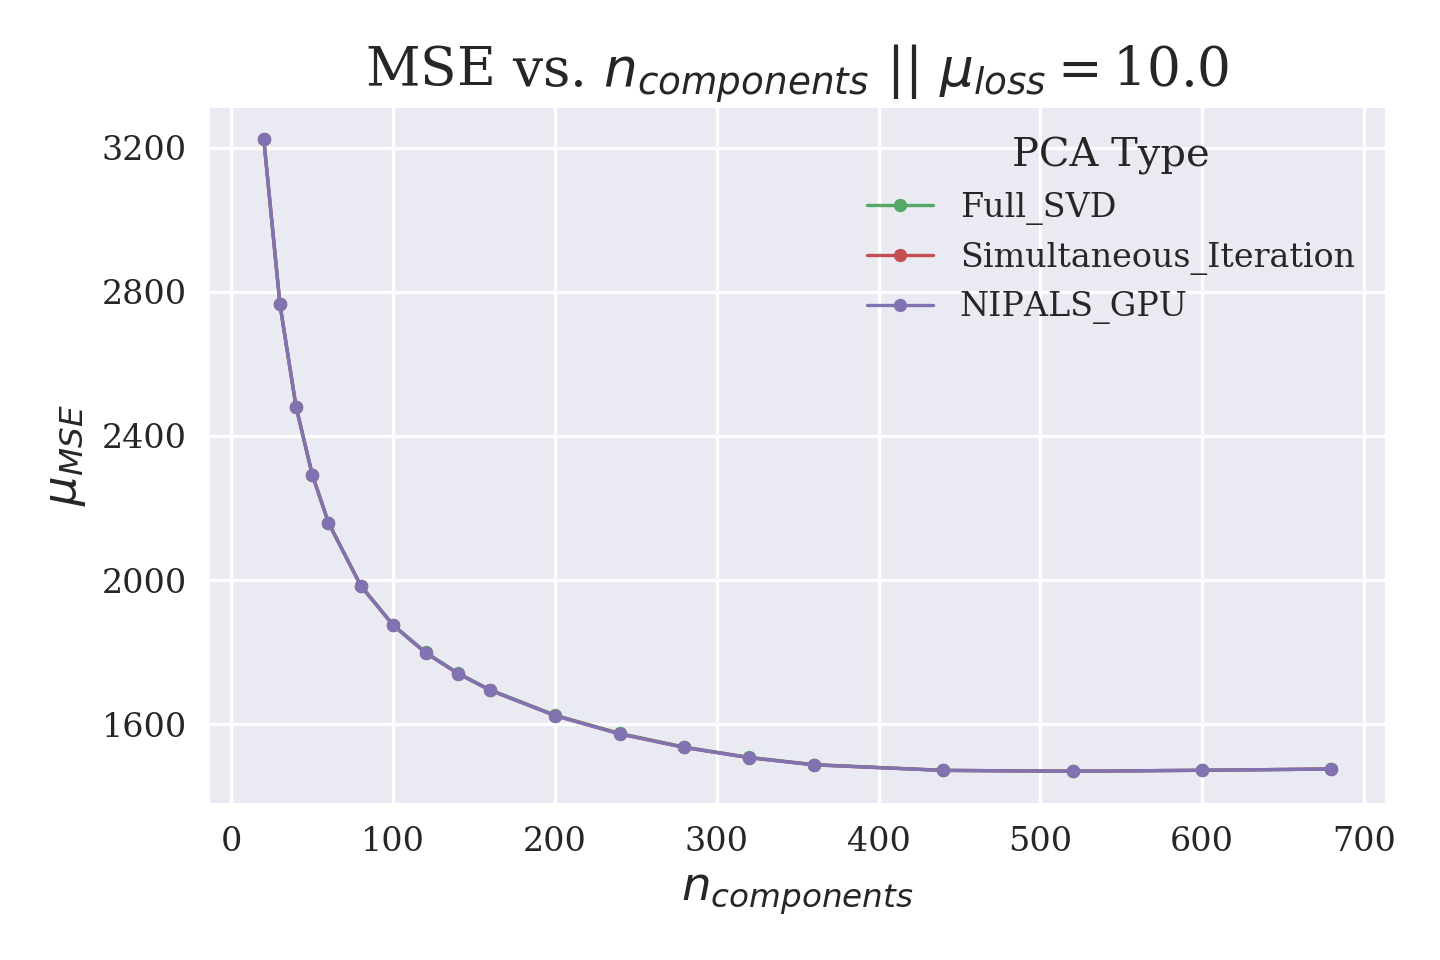
\includegraphics[width=\linewidth]{Noise10MSE.png}
  \captionof{figure}{The relationship between \textit{MSE} and $n_{components}$ for the dataset with $\mu_{noise} = 10$}
  \label{Noise10MSE}
\end{minipage}%
\quad
\begin{minipage}{.45\textwidth}
  \centering
  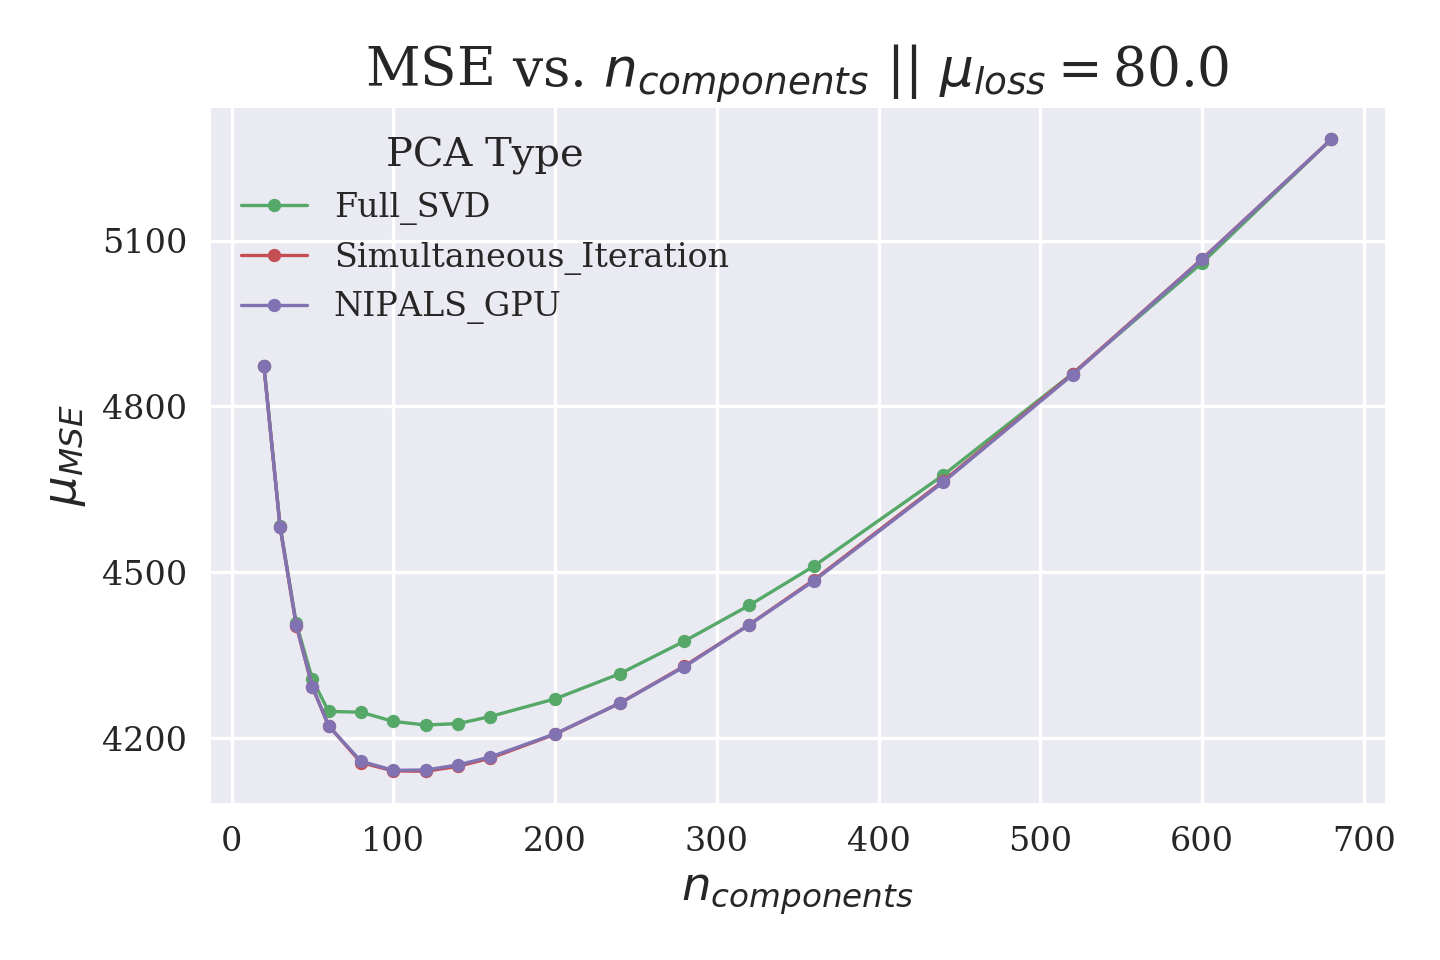
\includegraphics[width=\linewidth]{Noise80MSE.png}
  \captionof{figure}{The relationship between \textit{MSE} and $n_{components}$ for the dataset with $\mu_{noise} = 80$}
  \label{Noise80MSE}
\end{minipage}
\end{figure}

The three different PCA algorithms appear to perform nearly identically on the least noisy dataset, but for the noisiest dataset, there is a non-trivial difference between the algorithms. In particular, it appears that the de-noised images from the \textbf{\hyperref[3.2]{SVD}} algorithm are consistently more distant from the ground truth than the de-noised images from the other two variants.

Additionally, for the least noisy dataset, as $n_{components}$ increases, the value of $MSE$ generally decreases. However, for the dataset with $\mu_{noise}=80$ and the other high noise datasets, there appears to be an optimal value for $n_{components}$. That is, there is a definite minimum value of $n_{components}$ that minimizes the value of $MSE$. Therefore, we can conclude that the choice of $n_{components}$ not only has a significant impact on the algorithms' run-times but also has a large influence on the quality of images they produce.

%-----------------------------------------------------------------%
\subsection{Loss}\label{5.3}

As in the previous section, the obtained values of \textit{Loss} for both the lowest noise ($\mu_{noise}=10$) and highest noise ($\mu_{noise}=80$) datasets are shown below in \textbf{\hyperref[Noise10Loss]{Figures \ref*{Noise10Loss}}} and \textbf{\hyperref[Noise80Loss]{\ref*{Noise80Loss}}}, respectively.

\begin{figure}[H]
\centering
\begin{minipage}{.45\textwidth}
  \centering
  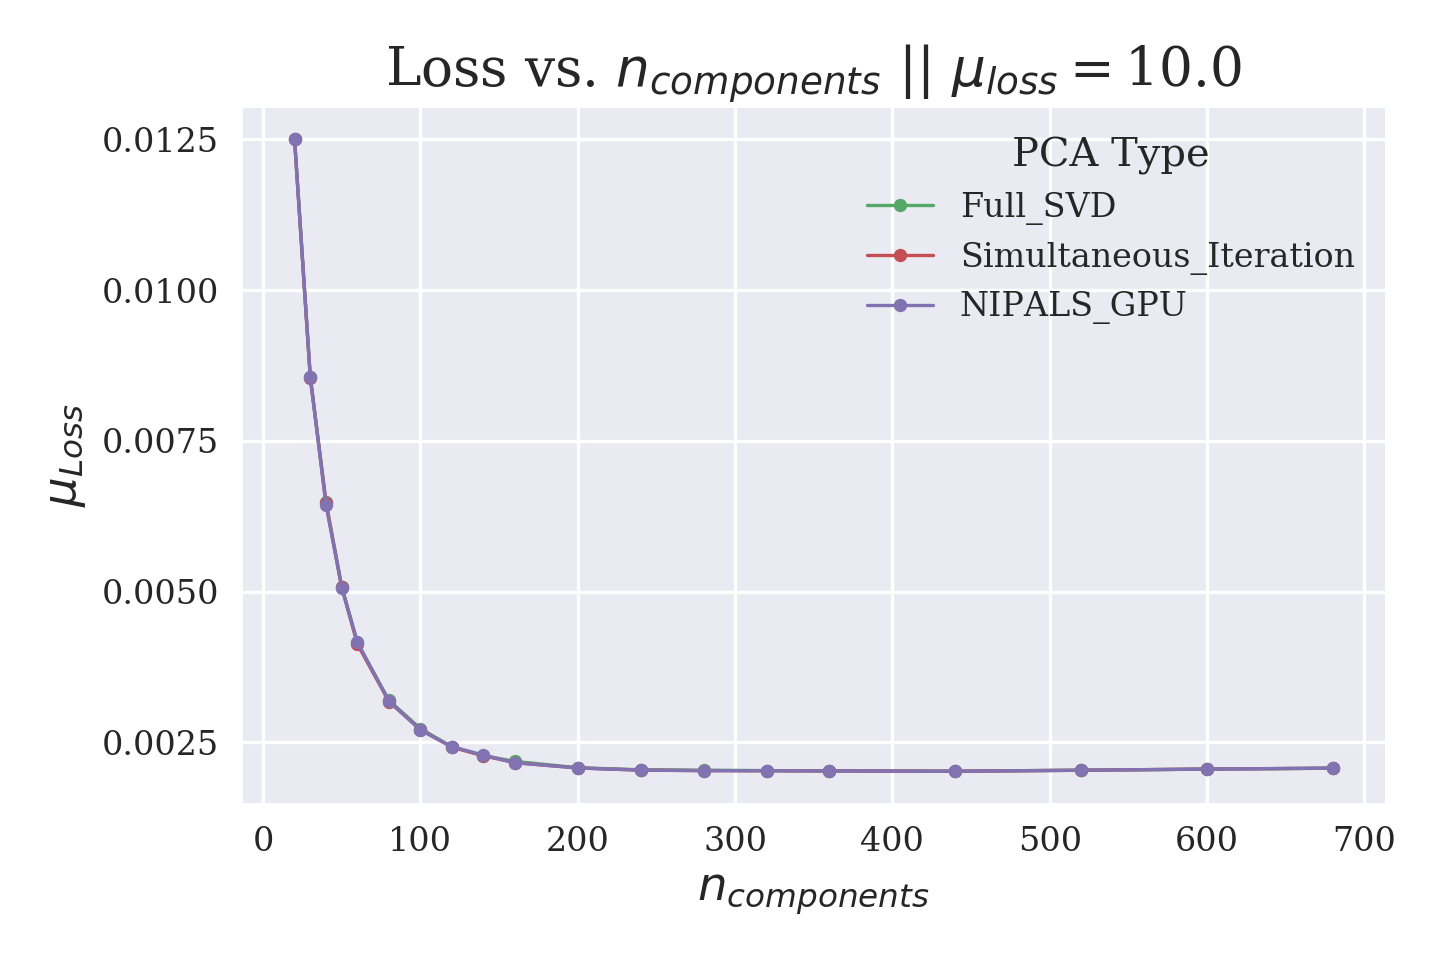
\includegraphics[width=\linewidth]{Noise10Loss.png}
  \captionof{figure}{The relationship between \textit{Loss} and $n_{components}$ for the dataset with $\mu_{noise} = 10$}
  \label{Noise10Loss}
\end{minipage}%
\quad
\begin{minipage}{.45\textwidth}
  \centering
  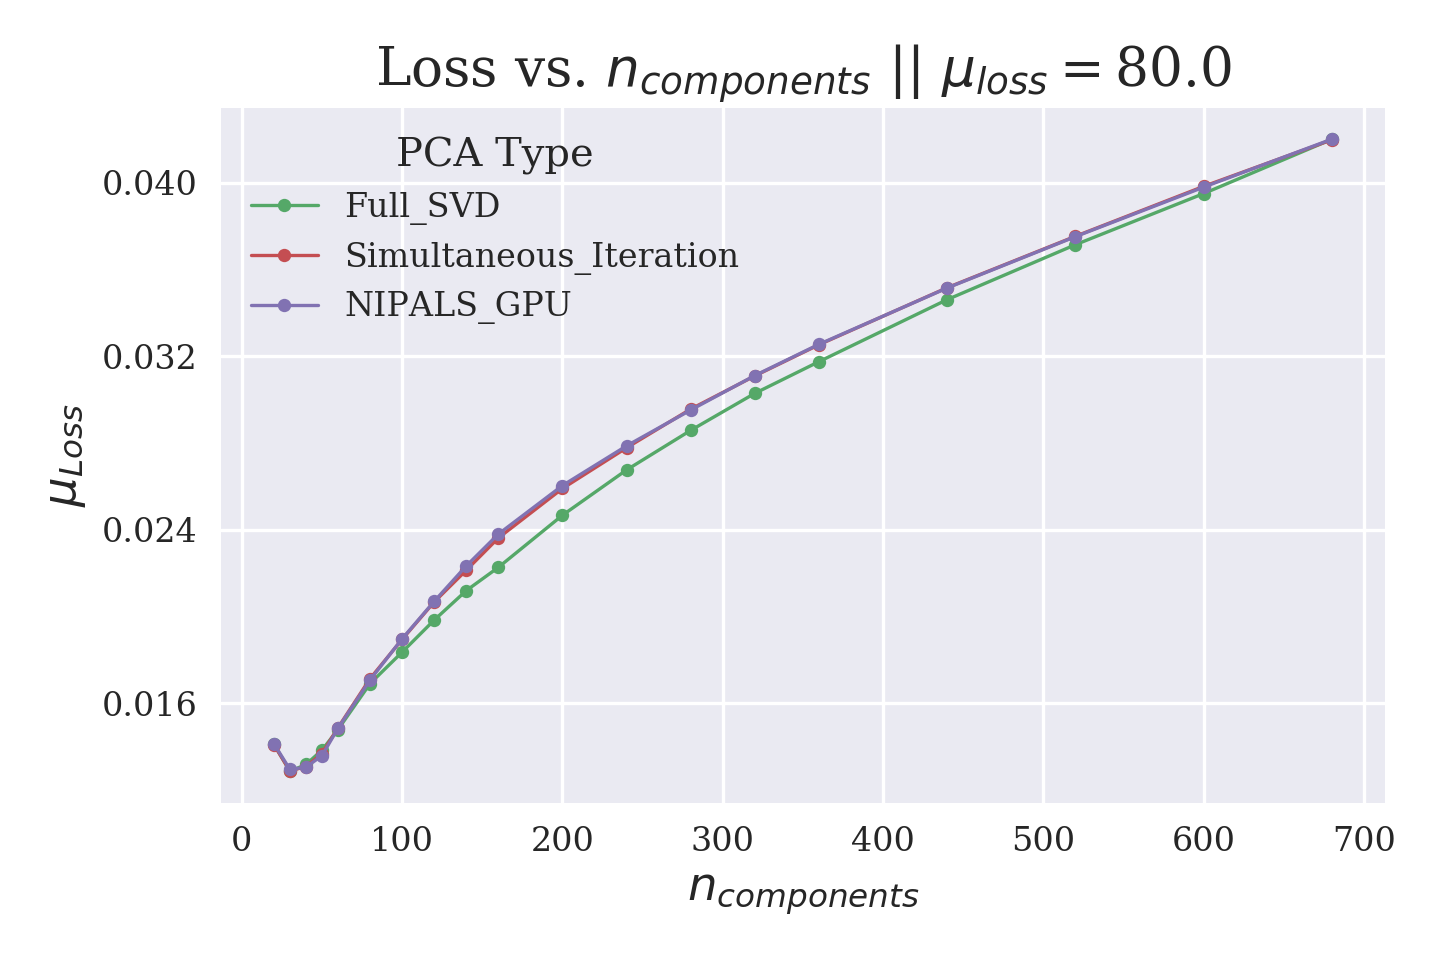
\includegraphics[width=\linewidth]{Noise80Loss.png}
  \captionof{figure}{The relationship between \textit{Loss} and $n_{components}$ for the dataset with $\mu_{noise} = 80$}
  \label{Noise80Loss}
\end{minipage}
\end{figure}

Like before, we see that the different PCA variants perform nearly identically for the lowest noise dataset. However, for the highest noise dataset something is quite different. Specifically, whereas before the \textbf{\hyperref[3.2]{SVD}} algorithm performed worse than its peers on the \textit{MSE} metric, on the \textit{Loss} metric, it appears to consistently perform the best out of the three. The reason for both of these discrepancies is unclear, though it may result from the small non-zero value added to the mean of both the \textbf{\hyperref[3.1]{NIPALS}} and  \textbf{\hyperref[3.3]{Simultaneous Iteration}} to prevent division by zero-norm vectors. In any case, we believe that the relative differences are not significant enough to have a noticeable impact on the algorithms' performance. 

Additionally, a curious difference in the optimal value of $n_{components}$ between the \textit{Loss} and \textit{MSE} metrics appears. In the case of \textit{Loss}, it appears that the optimal value is somewhat smaller and the local minimum somewhat steeper. This may result from the fact that classifiers are quite sensitive to the noise that a larger number of $n_{components}$ retains.

%-----------------------------------------------------------------%
\subsection{Error Rate}\label{5.4}

The data concerning the \textit{Error Rate}, again for the least and most noisy datasets are shown below in \textbf{\hyperref[Noise10Error]{Figures \ref*{Noise10Error}}} and \textbf{\hyperref[Noise80Error]{\ref*{Noise80Error}}}, respectively.

\begin{figure}[H]
\centering
\begin{minipage}{.45\textwidth}
  \centering
  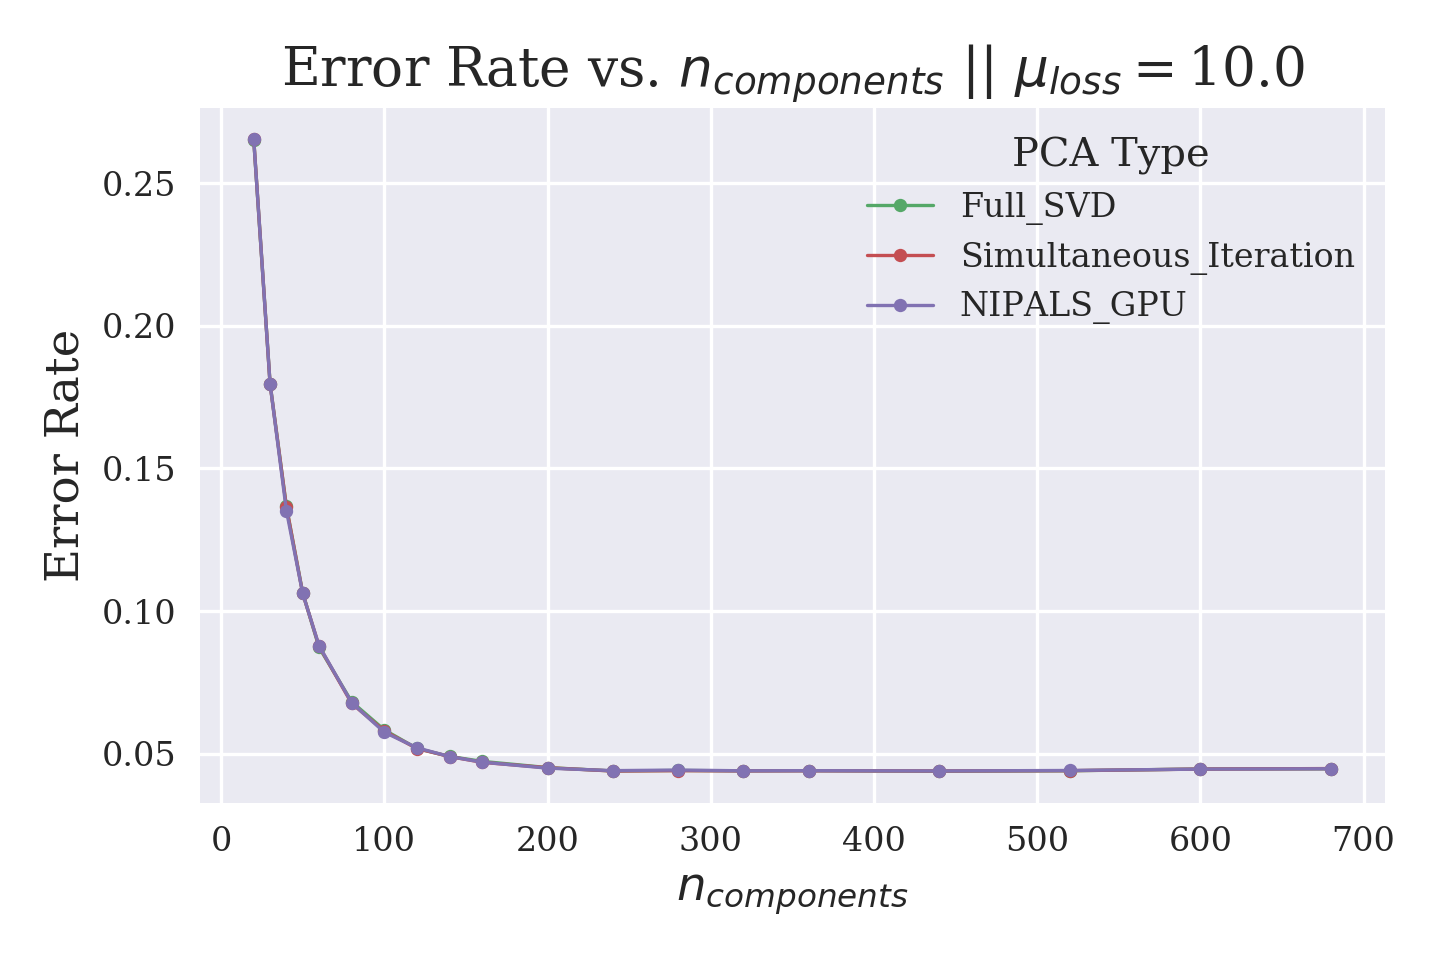
\includegraphics[width=\linewidth]{Noise10Error.png}
  \captionof{figure}{The relationship between \textit{Error Rate} and $n_{components}$ for the dataset with $\mu_{noise} = 10$}
  \label{Noise10Error}
\end{minipage}%
\quad
\begin{minipage}{.45\textwidth}
  \centering
  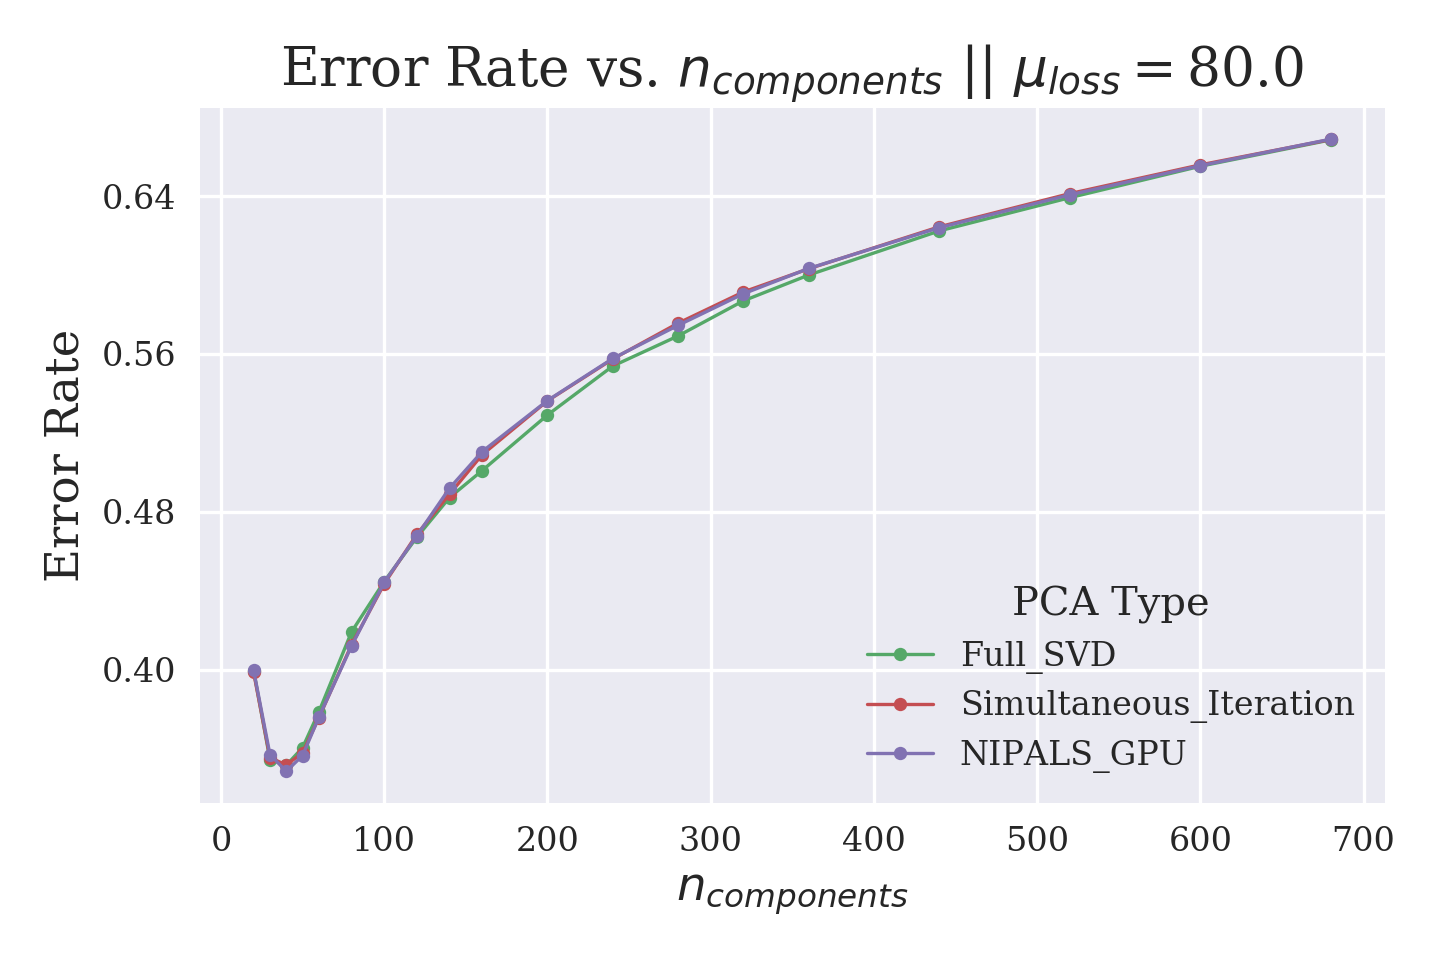
\includegraphics[width=\linewidth]{Noise80Error.png}
  \captionof{figure}{The relationship between \textit{Error Rate} and $n_{components}$ for the dataset with $\mu_{noise} = 80$}
  \label{Noise80Error}
\end{minipage}
\end{figure}

These results roughly mirror those concerning \textit{Loss}. This is hardly surprisingly, as the two metrics are inextricably linked by the classifiers. The main point of interest here is the fact that the relative discrepancy that was seen in the \textit{Loss} graphs is somewhat smaller in the \textit{Error Rate} graphs. This probably results from the fact that small changes in loss do not necessarily result in the re-classification of a sample.

%%%%%%%%%%%%%%%%%%%%%%%%%%%%%%%%%%%%%%%%%%%%%%%%%%%%%%%%%%%%%%%%%%%
%%%%%%%%%%%%%%%%%%%%%%%%%%%%%%%%%%%%%%%%%%%%%%%%%%%%%%%%%%%%%%%%%%%
\pagebreak
\section{Application to Classifier}\label{6}

In the \textbf{\hyperref[5.2]{analysis}} of the \textit{MSE} data, we noted that the ideal value of $n_{components}$ appears to vary with the magnitude of noise applied. We also noted that this value appears to change depending on the metric used. 

We show this below for all $8$ noise levels, using both \textit{MSE} and \textit{Loss}, in \textbf{\hyperref[MSE_All]{Figures \ref*{MSE_All}}} and \textbf{\hyperref[Loss_All]{\ref*{Loss_All}}}, respectively. Note that in these figures, the  metrics are averaged over both the $5$ classifiers and the $3$ different PCA methods.

\begin{figure}[H]
\centering
\begin{minipage}{.45\textwidth}
  \centering
  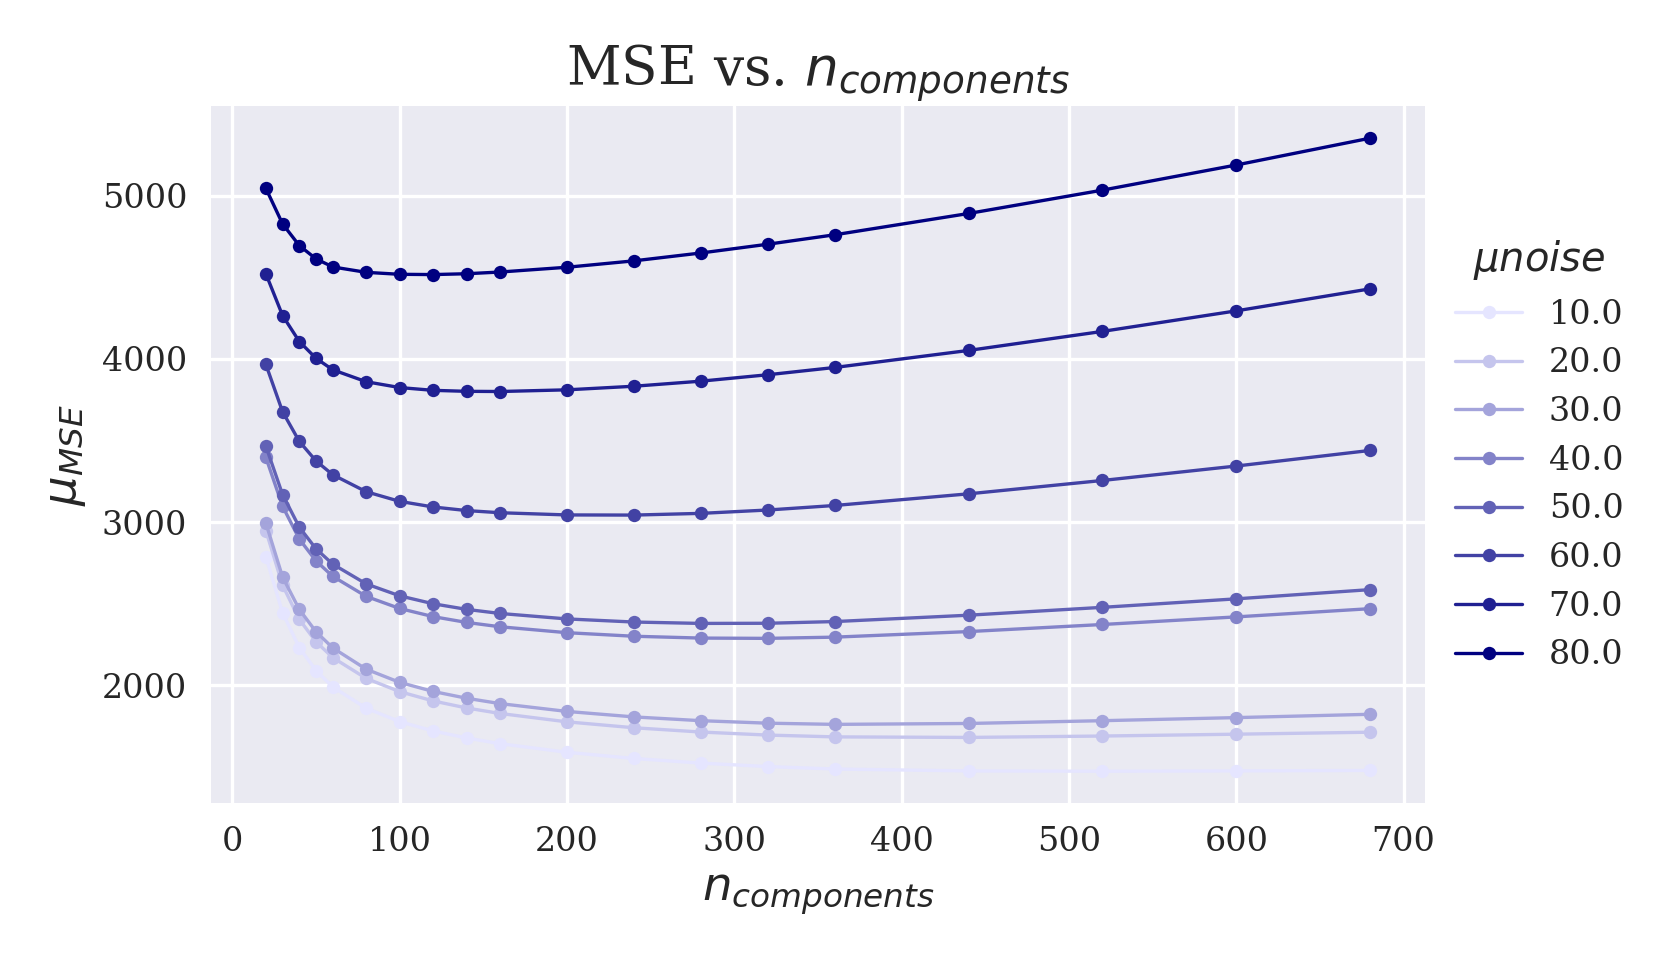
\includegraphics[width=\linewidth]{MSE_All.png}
  \captionof{figure}{The relationship between \textit{MSE} and $n_{components}$ for all $8$ noised datasets}
  \label{MSE_All}
\end{minipage}%
\quad
\begin{minipage}{.45\textwidth}
  \centering
  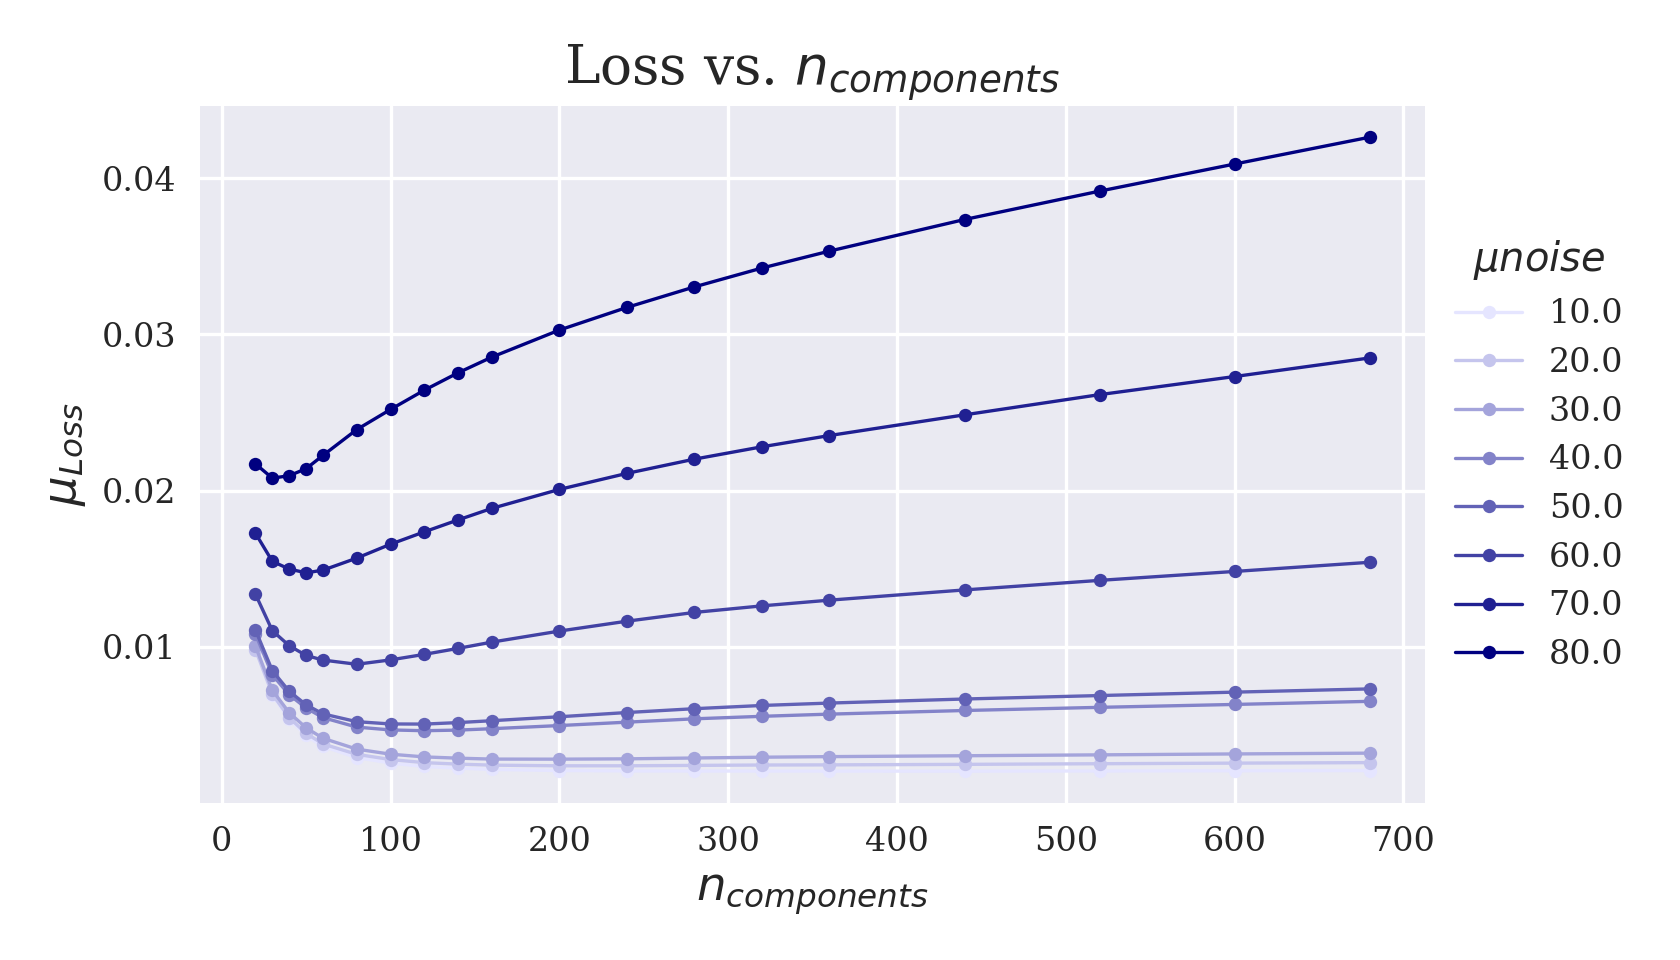
\includegraphics[width=\linewidth]{Loss_All.png}
  \captionof{figure}{The relationship between \textit{Loss} and $n_{components}$ for all $8$ noised datasets}
  \label{Loss_All}
\end{minipage}
\end{figure}

From these data, we can again determine that the optimal value of $n_{components}$ decreases as noise increases. And as before, we note that the curves for \textit{Loss} (and also for \textit{Error Rate}) reach their minimum earlier and are steeper than those relating to \textit{MSE}.

Nevertheless, since the end goal of using these PCA algorithms is to improve the performance of the classifier, we utilize the optimal value of $n_{components}$ with respect to \textit{Loss} in order to select the final PCA algorithm. In particular, for each noise value and each classifier, we select the value of $n_{components}$ that resulted in the lowest \textit{Loss} value. 

We give an example of how the selected PCA algorithms impact the classifiers' performances below in \textbf{\hyperref[PCA_Loss]{Figures \ref*{PCA_Loss}}} and \textbf{\hyperref[PCA_Error_Rate]{\ref*{PCA_Error_Rate}}} below, which show the average \textit{Loss} and \textit{Error Rate} respectively of the classifiers when each of the selected PCA algorithms is applied. The graphs also show the average performance of the classifiers on the raw noised data for comparison.

\begin{figure}[H]
\centering
\begin{minipage}{.45\textwidth}
  \centering
  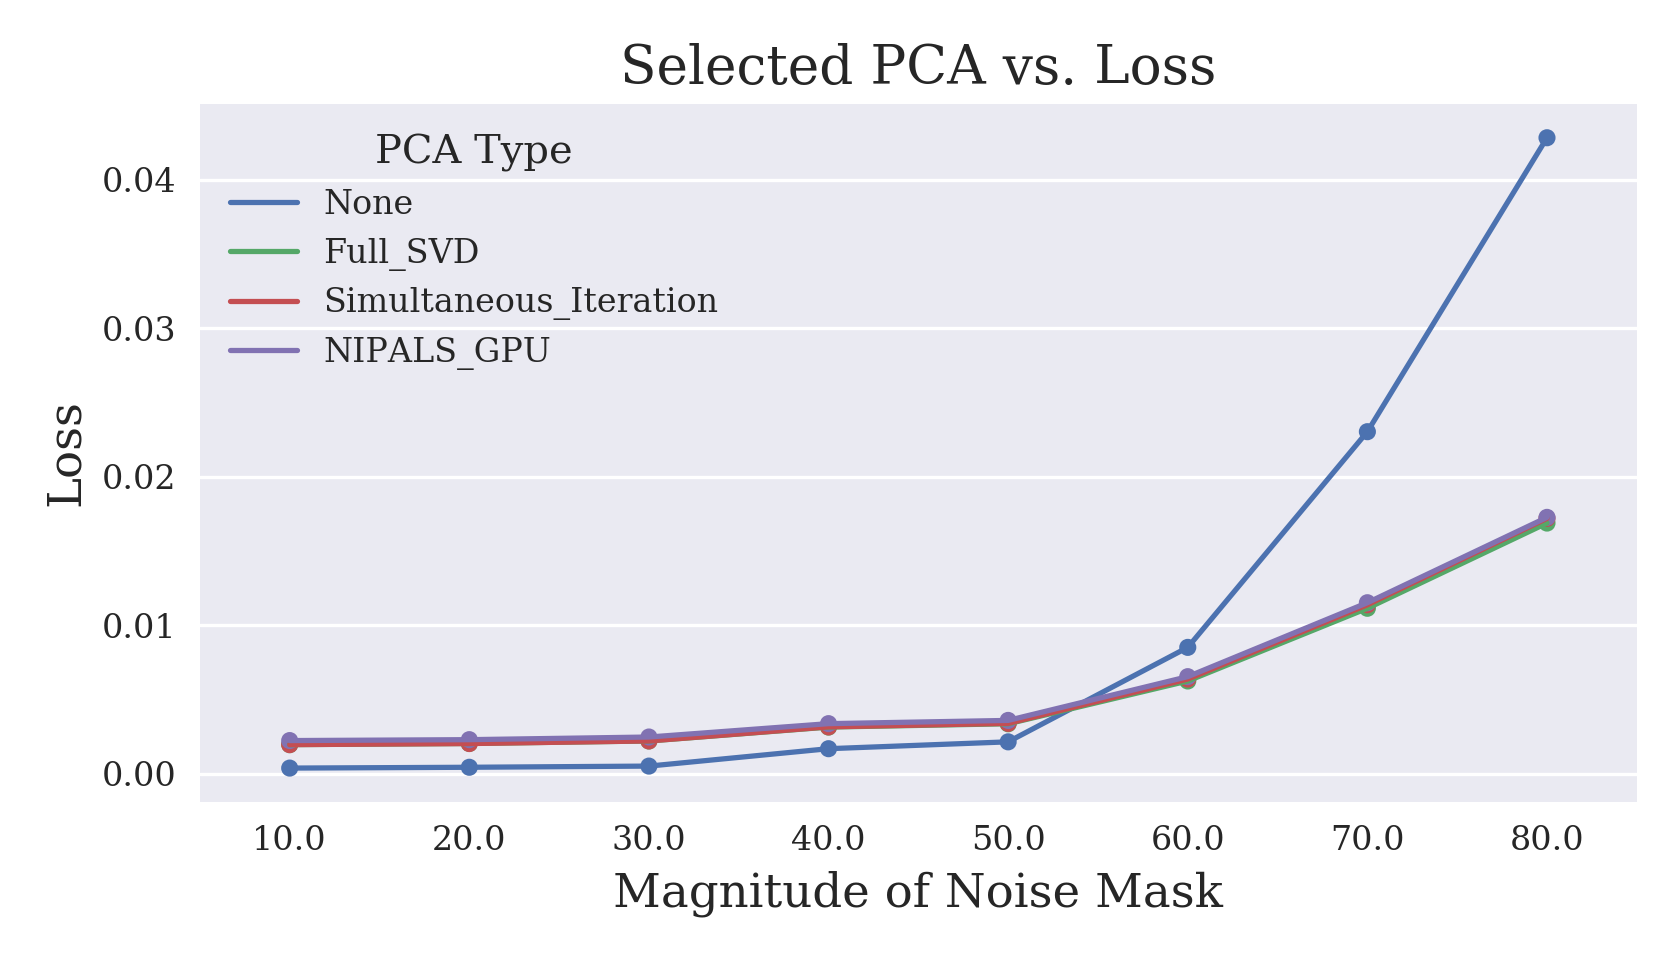
\includegraphics[width=\linewidth]{NIPALS_Loss.png}
  \captionof{figure}{The average \textit{Loss} of the classifiers when a PCA pre-processor is applied to the noised data}
  \label{PCA_Loss}
\end{minipage}%
\quad
\begin{minipage}{.45\textwidth}
  \centering
  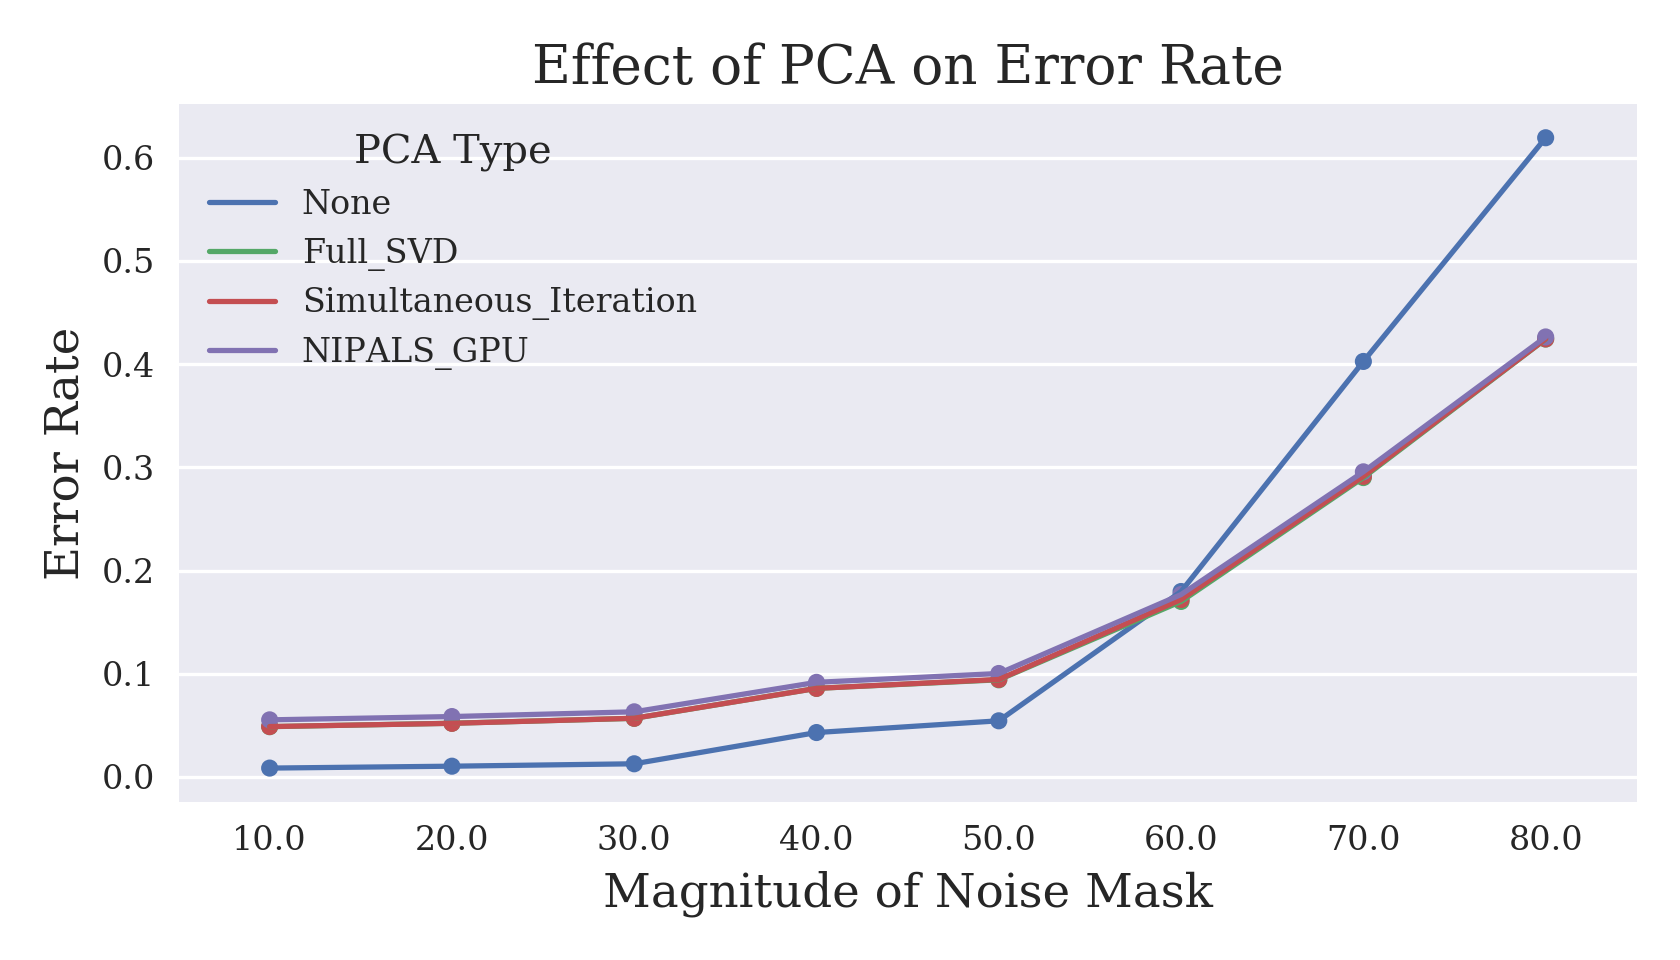
\includegraphics[width=\linewidth]{NIPALS_Error_Rate.png}
  \captionof{figure}{The average \textit{Error Rate} of the classifiers when a PCA pre-processor is applied to the noised data}
  \label{PCA_Error_Rate}
\end{minipage}
\end{figure}

The use of any of the three PCA algorithms results in roughly the same result in the classifier. Specifically, for lower values of noise, it appears that the use of a PCA pre-processor does not help the classifier at all; in fact, both the average \textit{Loss} and \textit{Error Rate} of the classifiers increases when the noise is low. However, at sufficiently high values of noise, it appears that using a PCA pre-processor has a significant positive impact on classifier performance. Indeed for the most noised data available, the use of any of the PCA algorithms resulted in a $>20\%$ increase in the accuracy of the classifier. And we surmise that if still more noise were to be added to the data, an even more significant difference could be observed. Hence, it appears that PCA can function as an image denoiser, particularly for data with extremely high levels of noise.


%%%%%%%%%%%%%%%%%%%%%%%%%%%%%%%%%%%%%%%%%%%%%%%%%%%%%%%%%%%%%%%%%%%
%%%%%%%%%%%%%%%%%%%%%%%%%%%%%%%%%%%%%%%%%%%%%%%%%%%%%%%%%%%%%%%%%%%
\pagebreak
\section{Conclusion}\label{7}

   Our results demonstrate that principal component analysis (PCA) can be an effective tool at de-noising images. Indeed, our data suggests that applying a PCA pre-processor to a set of noised images can significnatly improve data quality and aid in classification tasks, particularly when noise levels are significant. 
    
    Moreover, we find that while the output qualities of the three algorithms we analyzed, \textbf{\hyperref[3.1]{NIPALS}}, \textbf{\hyperref[3.2]{SVD}}, and \textbf{\hyperref[3.3]{Simultaneous Iteration}}, are quite similar, we find that their computaional complexity differs greatly. For image de-noising, due to the large number of components that need to be calculated, \textbf{\hyperref[3.2]{SVD}} appears to be by far the lowest in cost. Nevertheless, our results suggest that this will not always be the case, and in problems with different data requirements, one of the other variants may be the most efficient. 
    
    Finally, we raise several possible avenues of further research. One of the main characteristics of our approach to PCA is that it makes no assumptions about the input data. In particular, our PCA filter is not specific to a single classifier and relies only on the noised data. Tailoring PCA to the specific classification task, perhaps by including the unnoised training data may lead to larger improvements in classifier performance. Furthermore, the improvements in performance we found when converting \textit{NumPy} code to \textit{Numba}, and the speedups obtained by utilizing a GPU suggest that there are many options to further optimize implementations of the studied algorithms.


%%%%%%%%%%%%%%%%%%%%%%%%%%%%%%%%%%%%%%%%%%%%%%%%%%%%%%%%%%%%%%%%%%%
%%%%%%%%%%%%%%%%%%%%%%%%%%%%%%%%%%%%%%%%%%%%%%%%%%%%%%%%%%%%%%%%%%%
\pagebreak

\bibliographystyle{plain}

\bibliography{Bibliography}

%\printbibliography
\end{document}

%Tidbits
% The factor k converges in a manner proportion the %maximum of $$\frac{\lambda_n-\lambda_{n-1}}%{\lambda_n},\frac{\lambda_n}{\lambda_{n+1}}$$.